% Options for packages loaded elsewhere
% Options for packages loaded elsewhere
\PassOptionsToPackage{unicode}{hyperref}
\PassOptionsToPackage{hyphens}{url}
\PassOptionsToPackage{dvipsnames,svgnames,x11names}{xcolor}
%
\documentclass[
  letterpaper,
  DIV=11,
  numbers=noendperiod]{scrartcl}
\usepackage{xcolor}
\usepackage{amsmath,amssymb}
\setcounter{secnumdepth}{-\maxdimen} % remove section numbering
\usepackage{iftex}
\ifPDFTeX
  \usepackage[T1]{fontenc}
  \usepackage[utf8]{inputenc}
  \usepackage{textcomp} % provide euro and other symbols
\else % if luatex or xetex
  \usepackage{unicode-math} % this also loads fontspec
  \defaultfontfeatures{Scale=MatchLowercase}
  \defaultfontfeatures[\rmfamily]{Ligatures=TeX,Scale=1}
\fi
\usepackage{lmodern}
\ifPDFTeX\else
  % xetex/luatex font selection
\fi
% Use upquote if available, for straight quotes in verbatim environments
\IfFileExists{upquote.sty}{\usepackage{upquote}}{}
\IfFileExists{microtype.sty}{% use microtype if available
  \usepackage[]{microtype}
  \UseMicrotypeSet[protrusion]{basicmath} % disable protrusion for tt fonts
}{}
\makeatletter
\@ifundefined{KOMAClassName}{% if non-KOMA class
  \IfFileExists{parskip.sty}{%
    \usepackage{parskip}
  }{% else
    \setlength{\parindent}{0pt}
    \setlength{\parskip}{6pt plus 2pt minus 1pt}}
}{% if KOMA class
  \KOMAoptions{parskip=half}}
\makeatother
% Make \paragraph and \subparagraph free-standing
\makeatletter
\ifx\paragraph\undefined\else
  \let\oldparagraph\paragraph
  \renewcommand{\paragraph}{
    \@ifstar
      \xxxParagraphStar
      \xxxParagraphNoStar
  }
  \newcommand{\xxxParagraphStar}[1]{\oldparagraph*{#1}\mbox{}}
  \newcommand{\xxxParagraphNoStar}[1]{\oldparagraph{#1}\mbox{}}
\fi
\ifx\subparagraph\undefined\else
  \let\oldsubparagraph\subparagraph
  \renewcommand{\subparagraph}{
    \@ifstar
      \xxxSubParagraphStar
      \xxxSubParagraphNoStar
  }
  \newcommand{\xxxSubParagraphStar}[1]{\oldsubparagraph*{#1}\mbox{}}
  \newcommand{\xxxSubParagraphNoStar}[1]{\oldsubparagraph{#1}\mbox{}}
\fi
\makeatother


\usepackage{longtable,booktabs,array}
\usepackage{calc} % for calculating minipage widths
% Correct order of tables after \paragraph or \subparagraph
\usepackage{etoolbox}
\makeatletter
\patchcmd\longtable{\par}{\if@noskipsec\mbox{}\fi\par}{}{}
\makeatother
% Allow footnotes in longtable head/foot
\IfFileExists{footnotehyper.sty}{\usepackage{footnotehyper}}{\usepackage{footnote}}
\makesavenoteenv{longtable}
\usepackage{graphicx}
\makeatletter
\newsavebox\pandoc@box
\newcommand*\pandocbounded[1]{% scales image to fit in text height/width
  \sbox\pandoc@box{#1}%
  \Gscale@div\@tempa{\textheight}{\dimexpr\ht\pandoc@box+\dp\pandoc@box\relax}%
  \Gscale@div\@tempb{\linewidth}{\wd\pandoc@box}%
  \ifdim\@tempb\p@<\@tempa\p@\let\@tempa\@tempb\fi% select the smaller of both
  \ifdim\@tempa\p@<\p@\scalebox{\@tempa}{\usebox\pandoc@box}%
  \else\usebox{\pandoc@box}%
  \fi%
}
% Set default figure placement to htbp
\def\fps@figure{htbp}
\makeatother





\setlength{\emergencystretch}{3em} % prevent overfull lines

\providecommand{\tightlist}{%
  \setlength{\itemsep}{0pt}\setlength{\parskip}{0pt}}



 


\KOMAoption{captions}{tableheading}
\makeatletter
\@ifpackageloaded{caption}{}{\usepackage{caption}}
\AtBeginDocument{%
\ifdefined\contentsname
  \renewcommand*\contentsname{Table of contents}
\else
  \newcommand\contentsname{Table of contents}
\fi
\ifdefined\listfigurename
  \renewcommand*\listfigurename{List of Figures}
\else
  \newcommand\listfigurename{List of Figures}
\fi
\ifdefined\listtablename
  \renewcommand*\listtablename{List of Tables}
\else
  \newcommand\listtablename{List of Tables}
\fi
\ifdefined\figurename
  \renewcommand*\figurename{Figure}
\else
  \newcommand\figurename{Figure}
\fi
\ifdefined\tablename
  \renewcommand*\tablename{Table}
\else
  \newcommand\tablename{Table}
\fi
}
\@ifpackageloaded{float}{}{\usepackage{float}}
\floatstyle{ruled}
\@ifundefined{c@chapter}{\newfloat{codelisting}{h}{lop}}{\newfloat{codelisting}{h}{lop}[chapter]}
\floatname{codelisting}{Listing}
\newcommand*\listoflistings{\listof{codelisting}{List of Listings}}
\makeatother
\makeatletter
\makeatother
\makeatletter
\@ifpackageloaded{caption}{}{\usepackage{caption}}
\@ifpackageloaded{subcaption}{}{\usepackage{subcaption}}
\makeatother
\usepackage{bookmark}
\IfFileExists{xurl.sty}{\usepackage{xurl}}{} % add URL line breaks if available
\urlstyle{same}
\hypersetup{
  pdftitle={Exploratory Analysis of NVSS Multiple Cause-of-Death Mortality Data},
  pdfauthor={Carol Xu},
  colorlinks=true,
  linkcolor={blue},
  filecolor={Maroon},
  citecolor={Blue},
  urlcolor={Blue},
  pdfcreator={LaTeX via pandoc}}


\title{Exploratory Analysis of NVSS Multiple Cause-of-Death Mortality
Data}
\author{Carol Xu}
\date{}
\begin{document}
\maketitle

\renewcommand*\contentsname{Table of contents}
{
\hypersetup{linkcolor=}
\setcounter{tocdepth}{2}
\tableofcontents
}

\subsection{Total Overdose Deaths in the U.S.
(1999-2020)}\label{total-overdose-deaths-in-the-u.s.-1999-2020}

Overdose deaths defined by the following ICD-10 Underlying Cause of
Death (UCOD) codes:

Code

Description

X40--X44

Unintentional/Accidental poisoning by drugs and other biological
substances

X60--X64

Suicide/Intentional self-poisoning by drugs and other biological
substances

X85

Assault/Homicide by drugs, biological substances, and other substances

Y10--Y14

Undetermined intent, Poisoning by drugs and biological substances

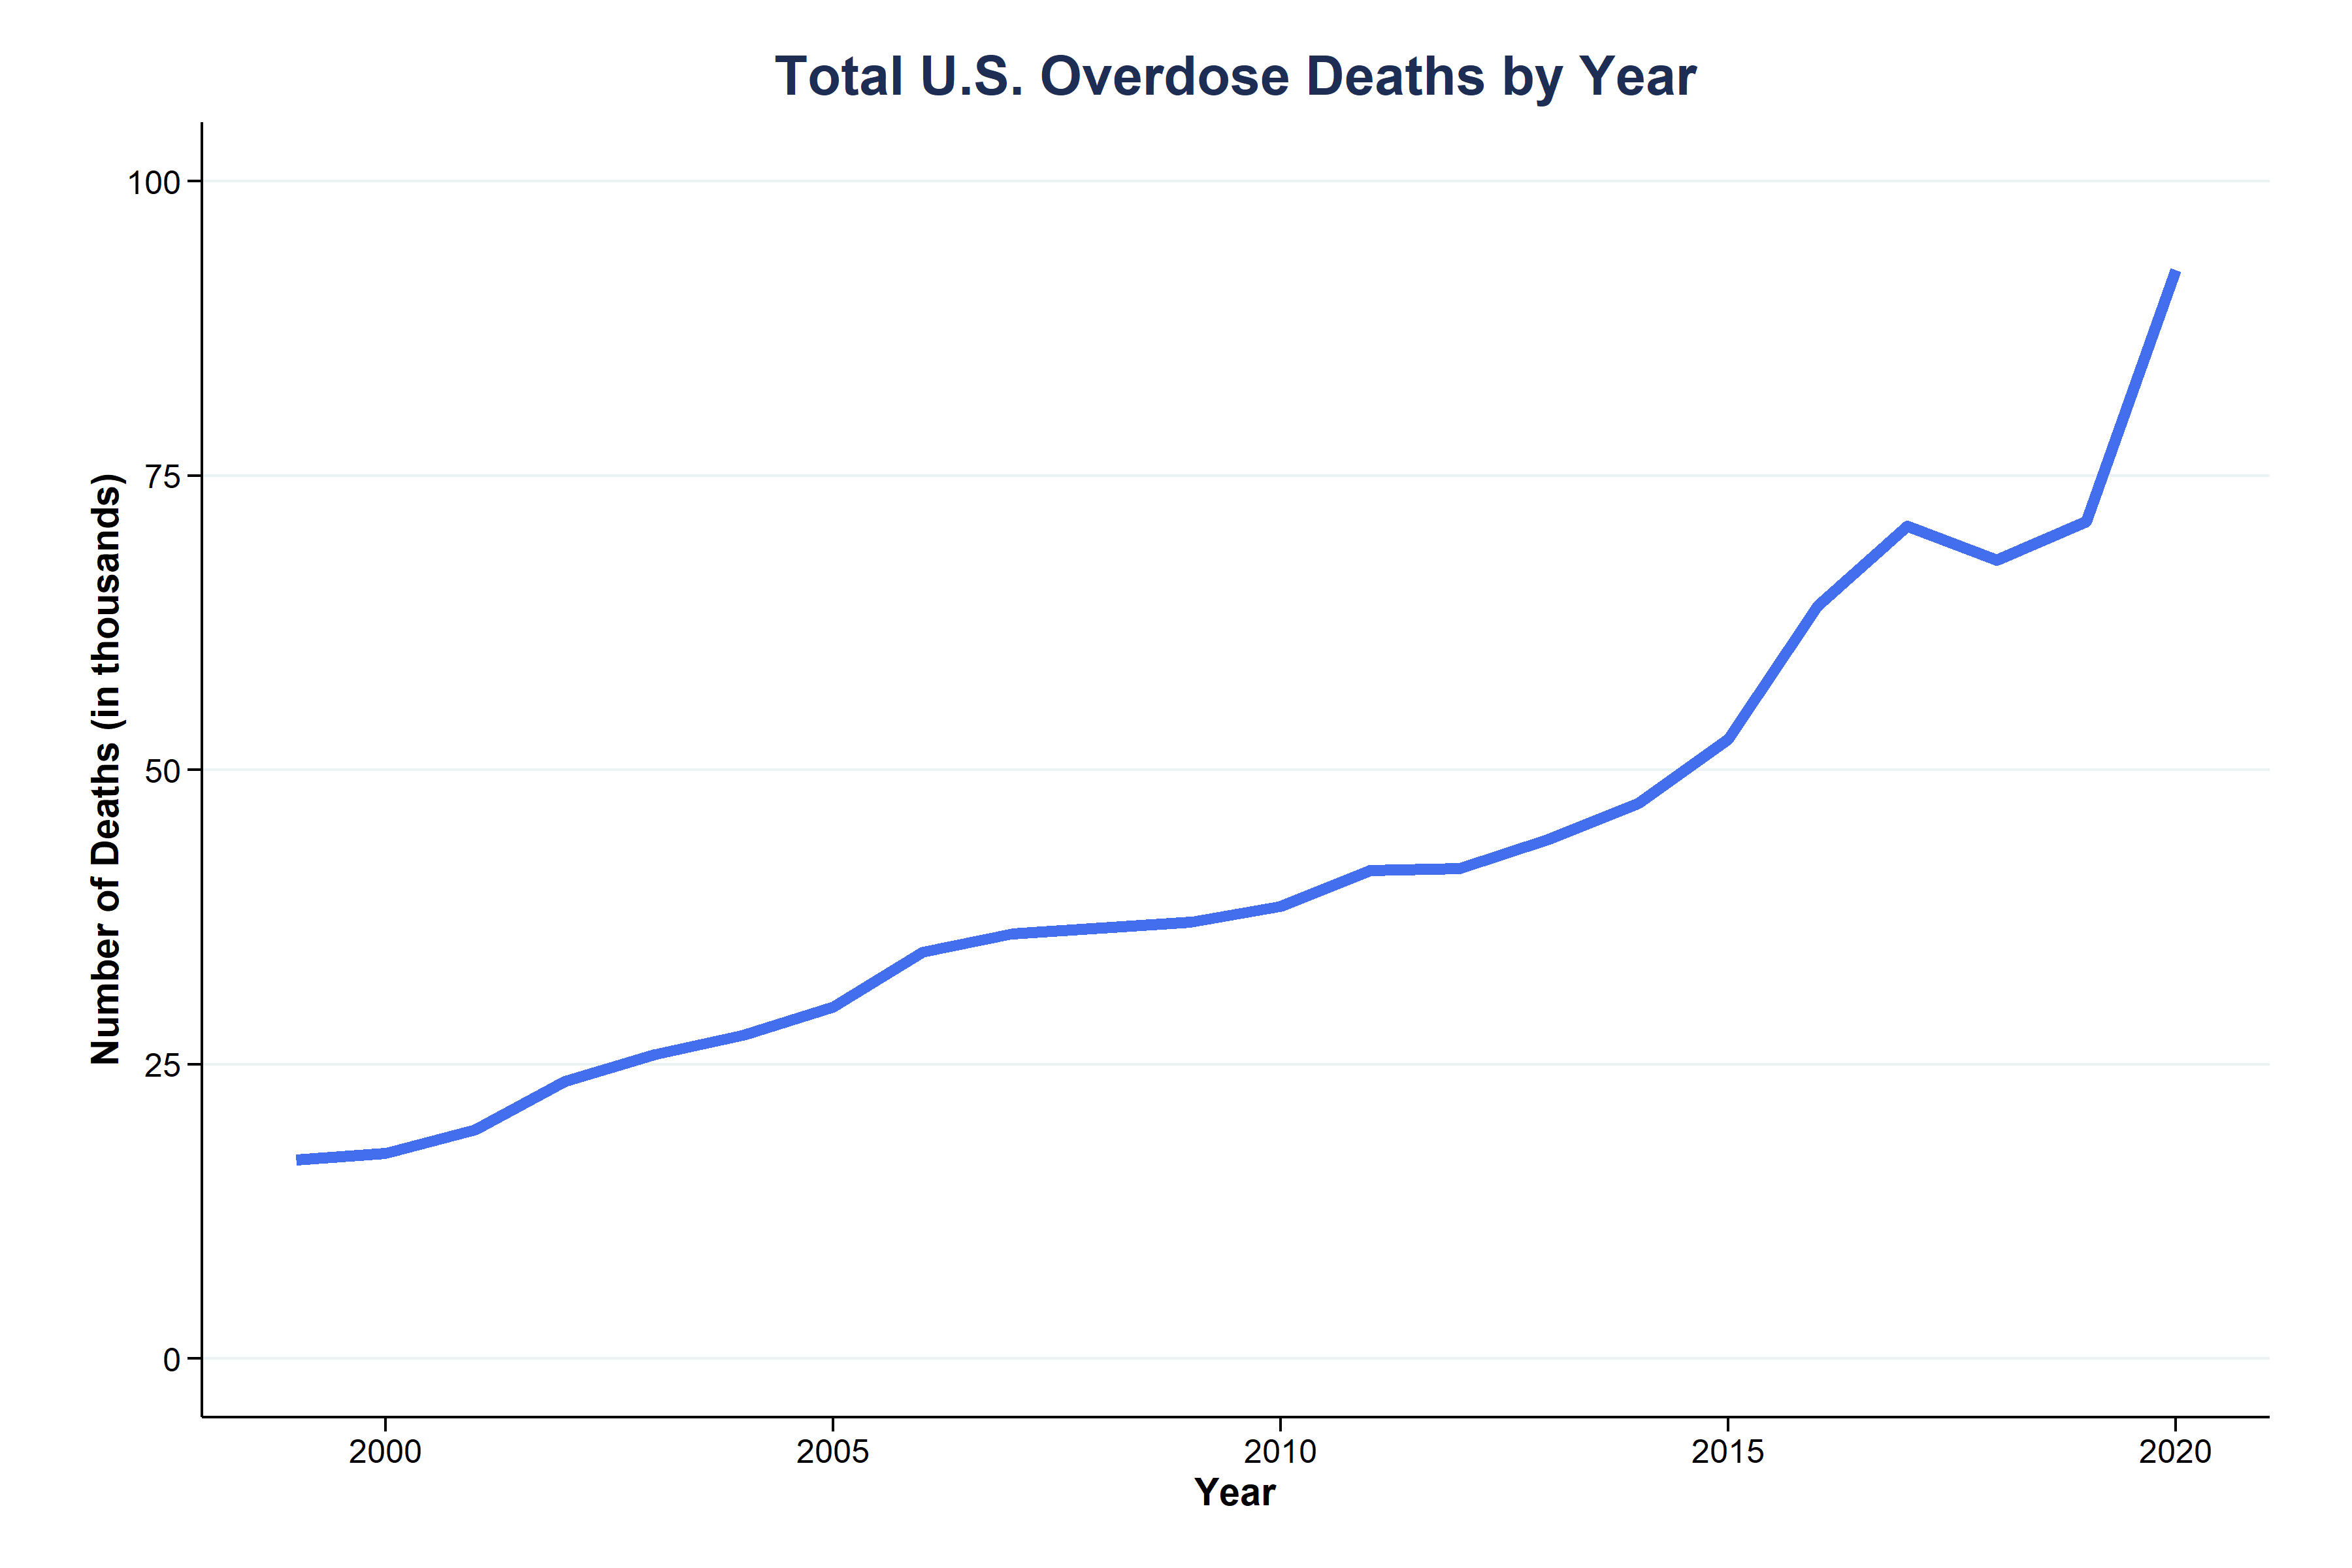
\includegraphics[width=0.8\linewidth,height=\textheight,keepaspectratio]{overdose_deaths_by_year.png}

\paragraph{n = 936,279}\label{n-936279}

\pandocbounded{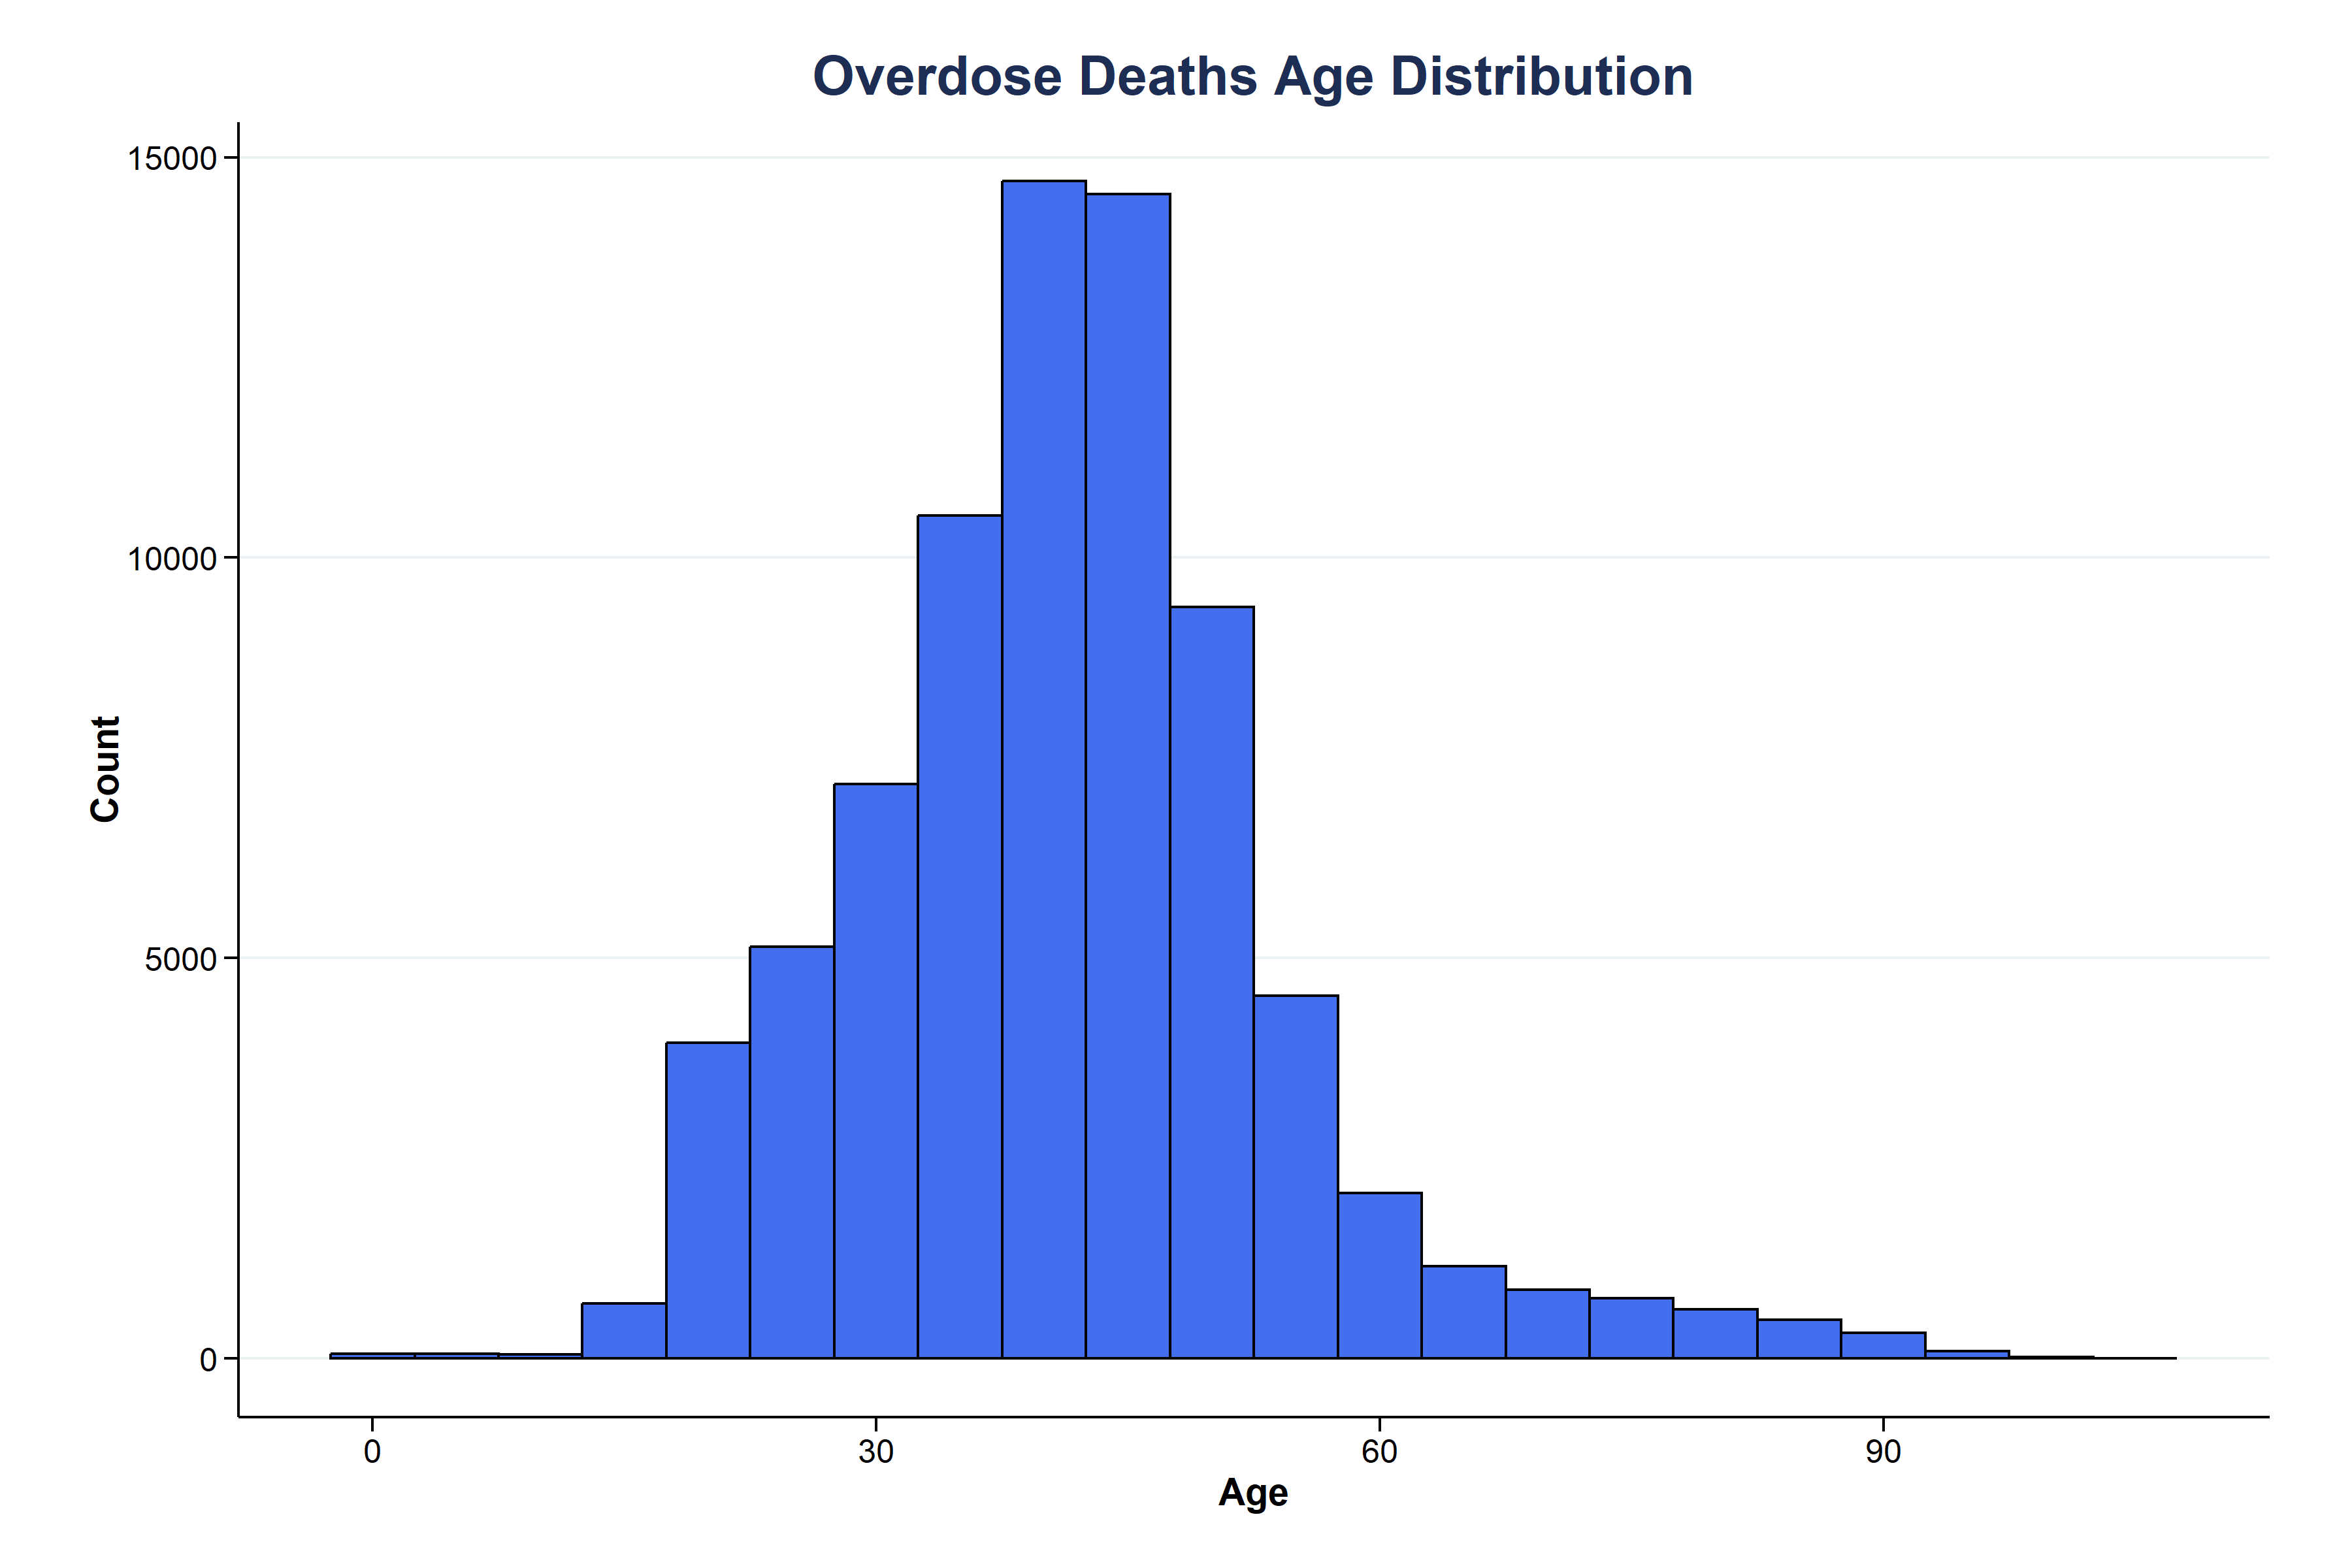
\includegraphics[keepaspectratio]{age.png}}

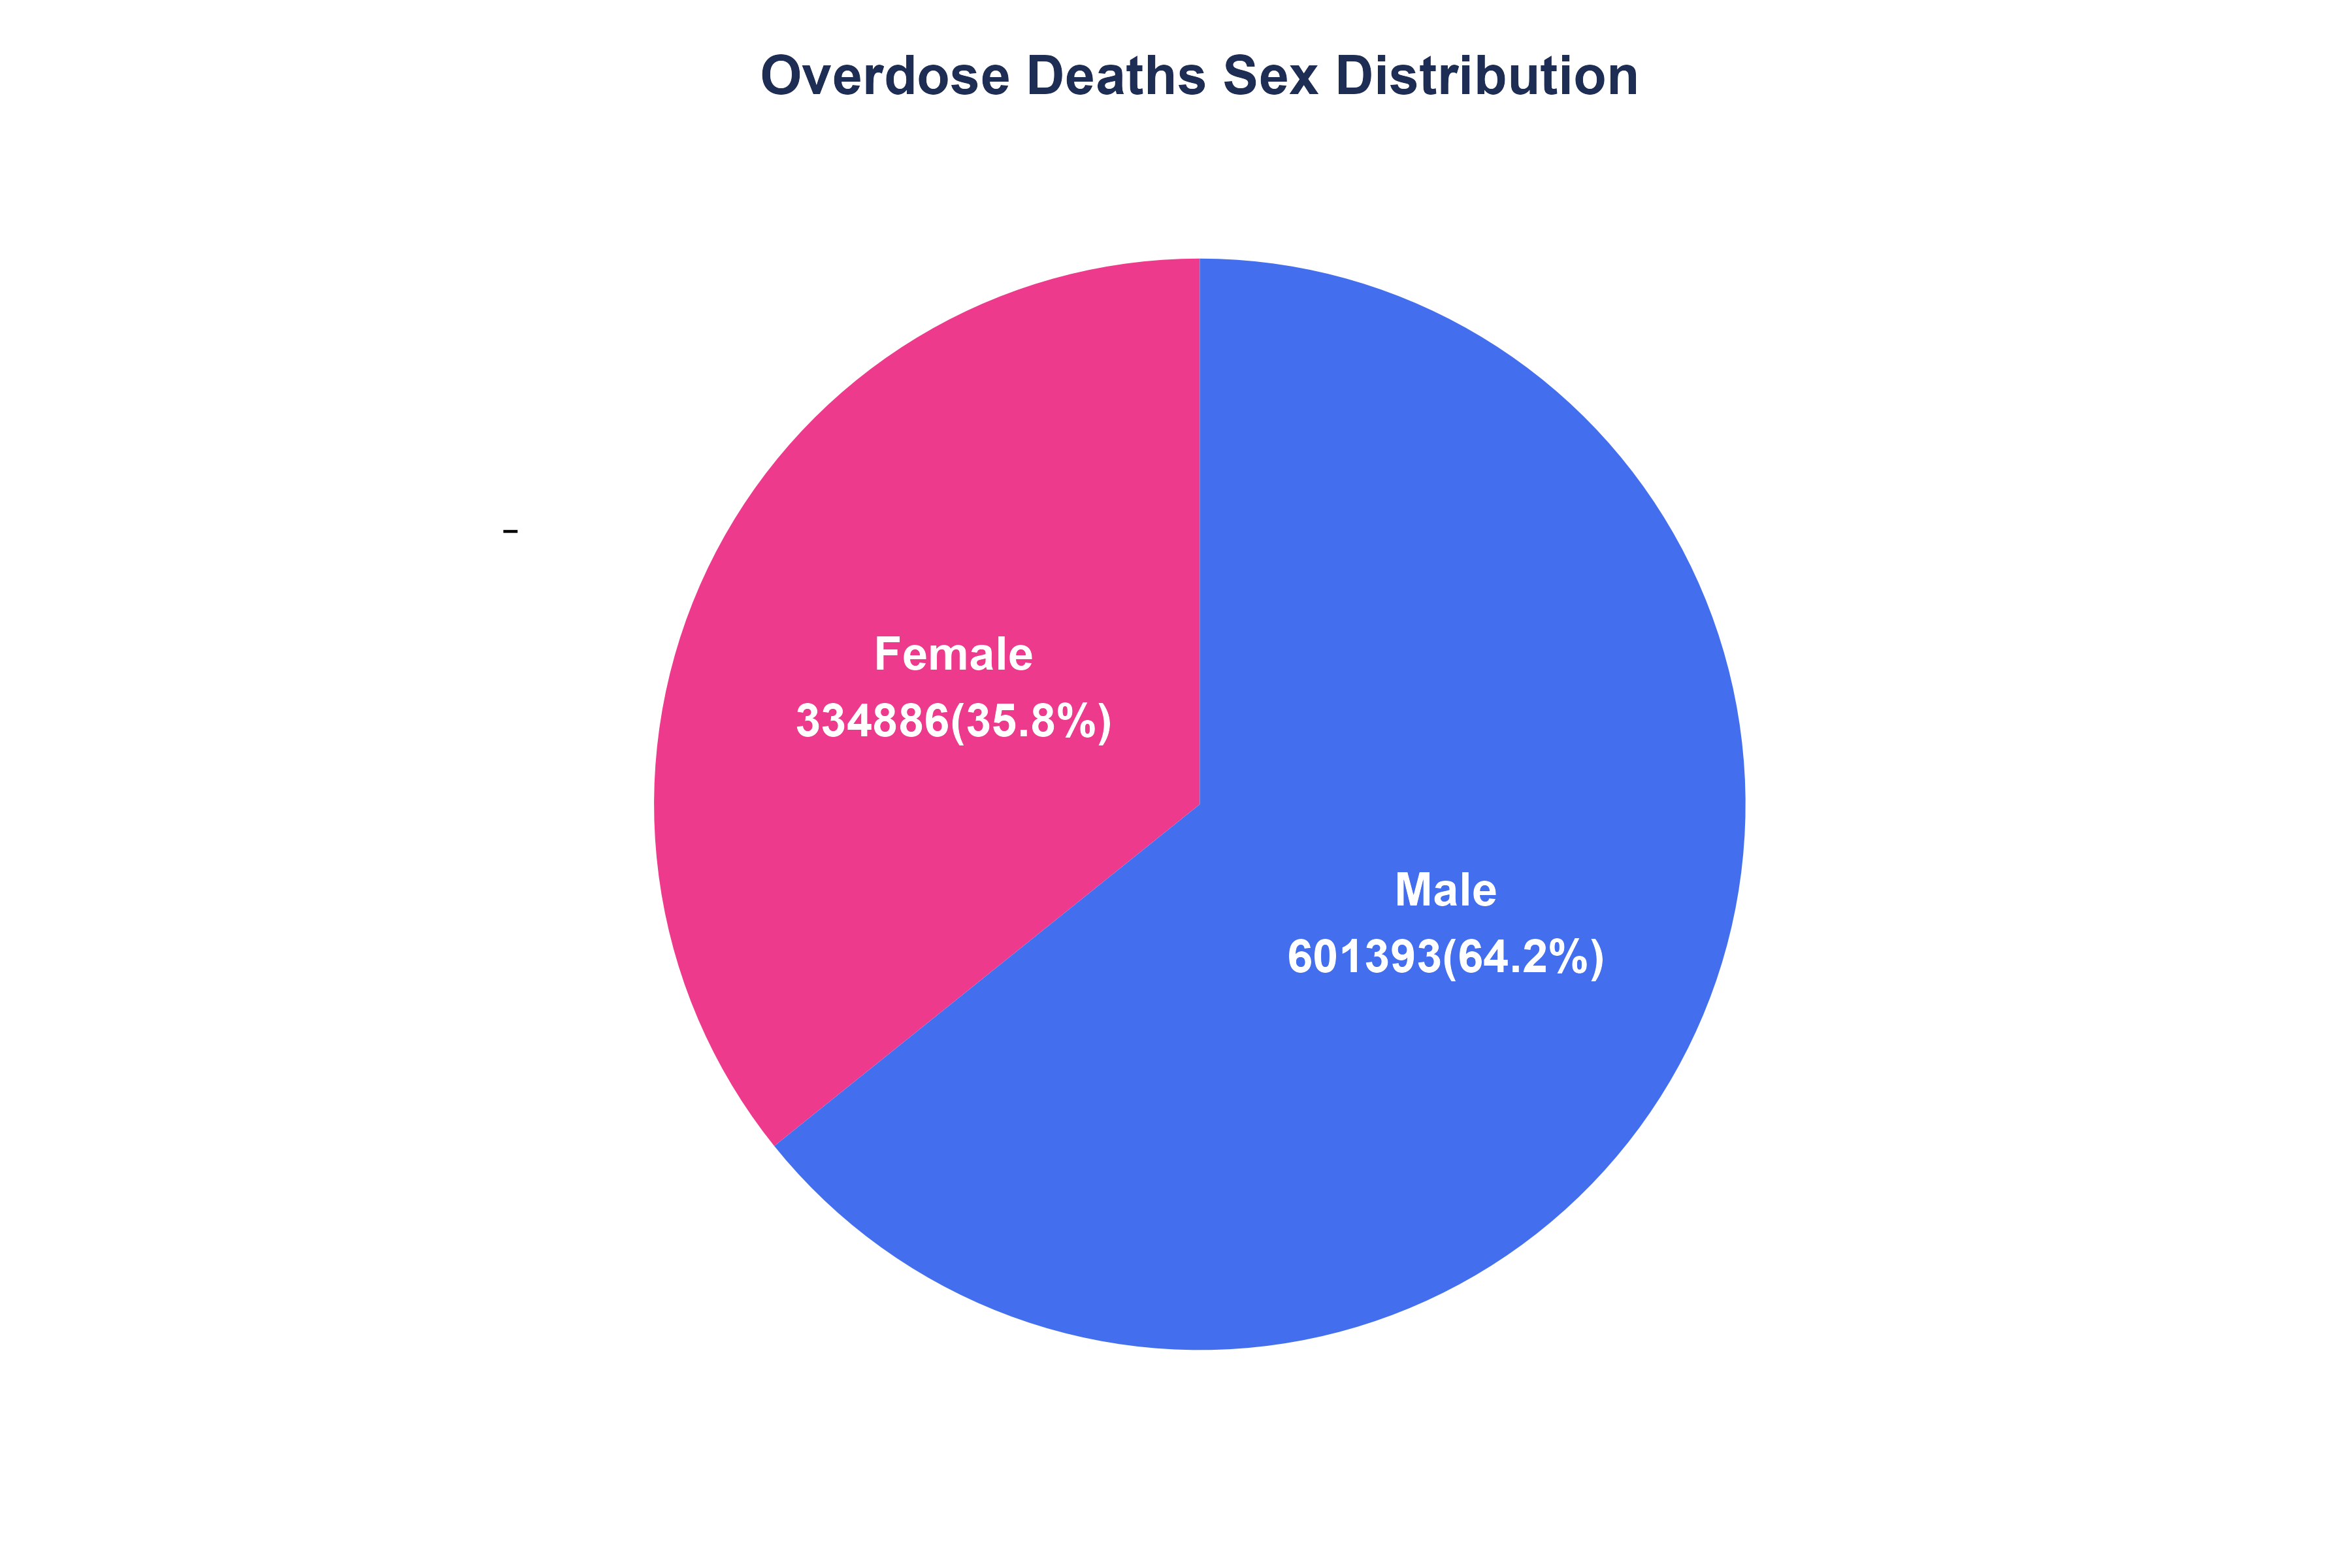
\includegraphics[width=1\linewidth,height=\textheight,keepaspectratio]{sex.png}

\subsection{Top 10 ICD-10 Codes
(1999-2020)}\label{top-10-icd-10-codes-1999-2020}

See
\href{https://github.com/carol-xu4/mortality/tree/main/results/top_icd-10_tables}{\texttt{results/top\_icd-10\_tables}}
for top 20 ICD-10 codes in each year.

\begin{longtable}[]{@{}
  >{\raggedright\arraybackslash}p{(\linewidth - 4\tabcolsep) * \real{0.0984}}
  >{\raggedright\arraybackslash}p{(\linewidth - 4\tabcolsep) * \real{0.1148}}
  >{\raggedright\arraybackslash}p{(\linewidth - 4\tabcolsep) * \real{0.7869}}@{}}
\toprule\noalign{}
\begin{minipage}[b]{\linewidth}\raggedright
Rank
\end{minipage} & \begin{minipage}[b]{\linewidth}\raggedright
Code
\end{minipage} & \begin{minipage}[b]{\linewidth}\raggedright
Description
\end{minipage} \\
\midrule\noalign{}
\endhead
\bottomrule\noalign{}
\endlastfoot
1 & T509 & Other and unspecified drugs/medicaments (Acidifying agents,
Alkalyzing agents, Immunoglobulin, Immunologicals, Lipotropic drugs,
Parathyroid hormones and derivatives) \\
2 & X42 & Accidental poisoning by narcotics/psychodysleptics (Incl.
Cannabis, Cocaine, Codeine, Heroin, Lysergide, Mescaline, Methadone,
Morphine, Opium) \\
3 & X44 & Accidental poisoning (unspecified drugs) \\
4 & T404 & Other synthetic narcotics (Pethidine) \\
5 & T402 & Other opioids (Codeine, Morphine) \\
6 & T405 & Cocaine \\
7 & T401 & Heroin \\
8 & F191 & Mental/behavioral disorders due to psychoactive substance use
(Harmful use) \\
9 & T424 & Benzodiazepines \\
10 & T436 & Psychostimulants with abuse potential \\
\end{longtable}

This summary is not a unique number of deaths; Number of occurrences
includes duplicates, for death certificates with multiple ICD-10 codes.

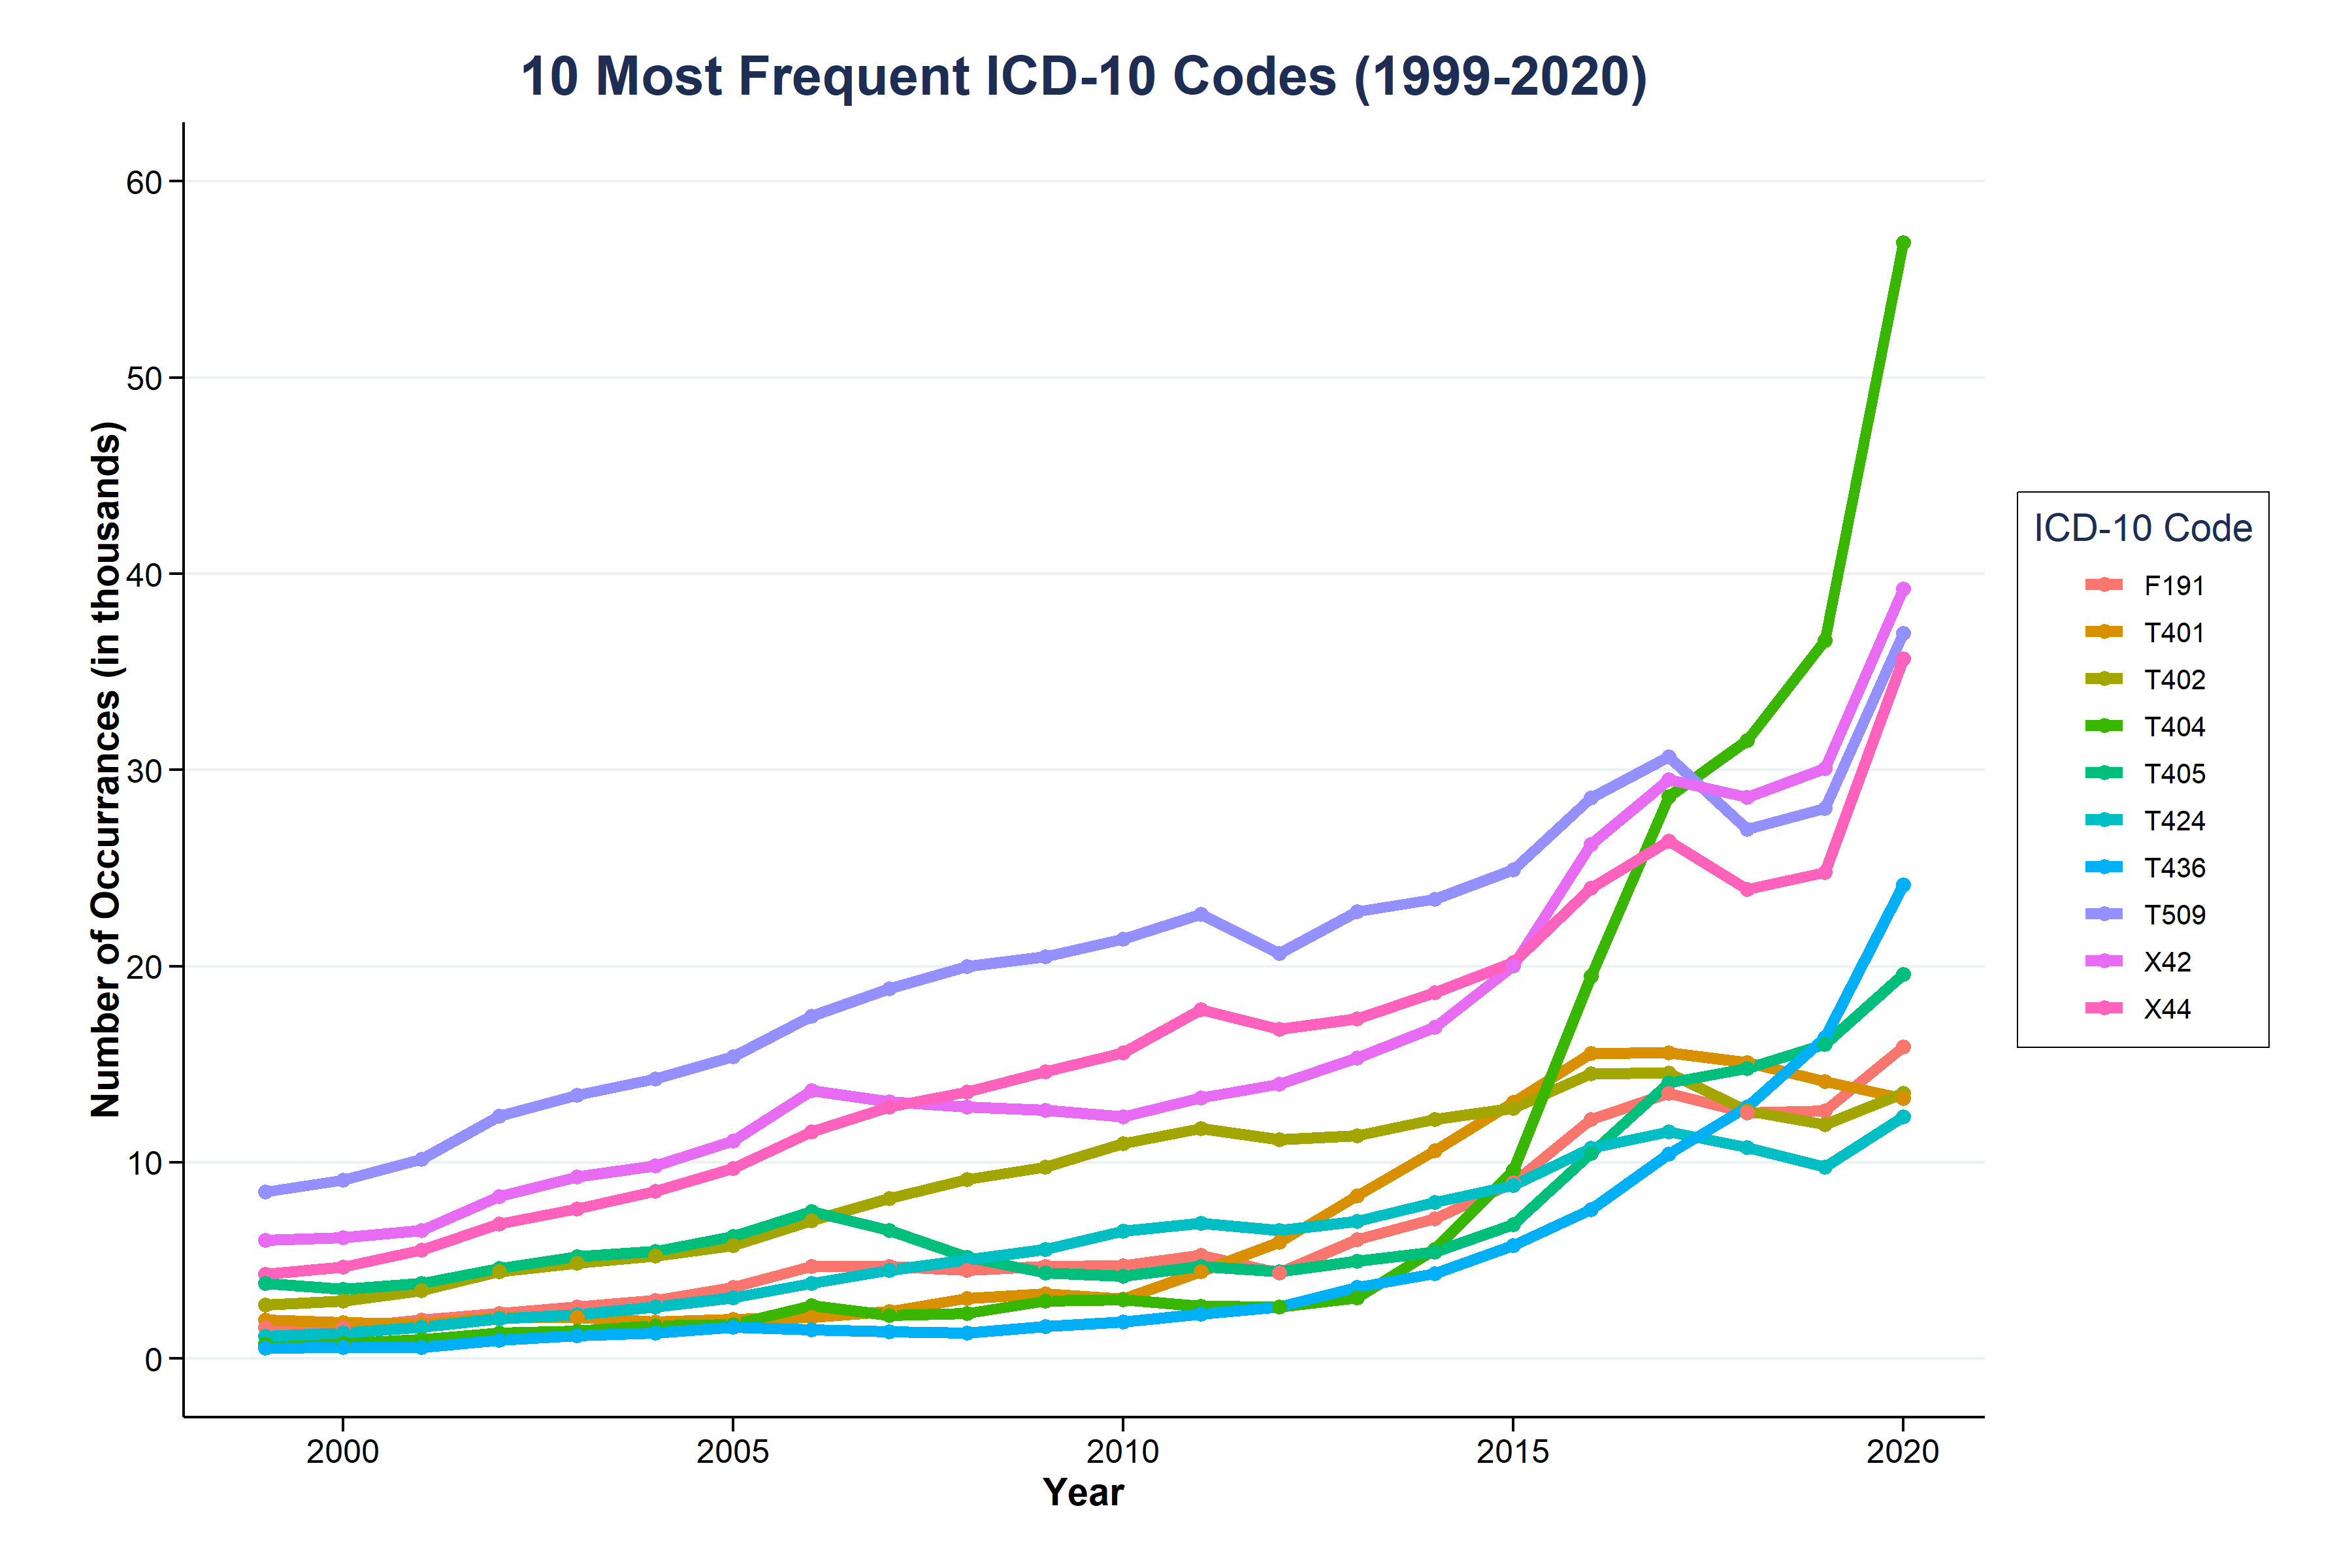
\includegraphics[width=0.9\linewidth,height=\textheight,keepaspectratio]{topicd.png}

\subsection{Substances of Interest (ICD-10
Codes)}\label{substances-of-interest-icd-10-codes}

\begin{longtable}[]{@{}ll@{}}
\toprule\noalign{}
Code & Substance \\
\midrule\noalign{}
\endhead
\bottomrule\noalign{}
\endlastfoot
\textbf{Opioids} & \\
T40.0 & Opium \\
T40.1 & Heroin \\
T40.2 & Other opioids (morphine, codeine) \\
T40.3 & Methadone \\
T40.4 & Synthetic narcotics (pethidine, fentanyl, etc.) \\
\textbf{Stimulants} & \\
T40.5 & Cocaine \\
T43.6 & Methamphetamine / other psychostimulants \\
\textbf{Depressants (non-opioid) / Sedatives} & \\
T42.3 & Barbiturates \\
T42.4 & Benzodiazepines \\
\textbf{Other} & \\
T40.7 & Cannabis (derivatives) \\
\end{longtable}

\subsection{Opioids}\label{opioids}

\pandocbounded{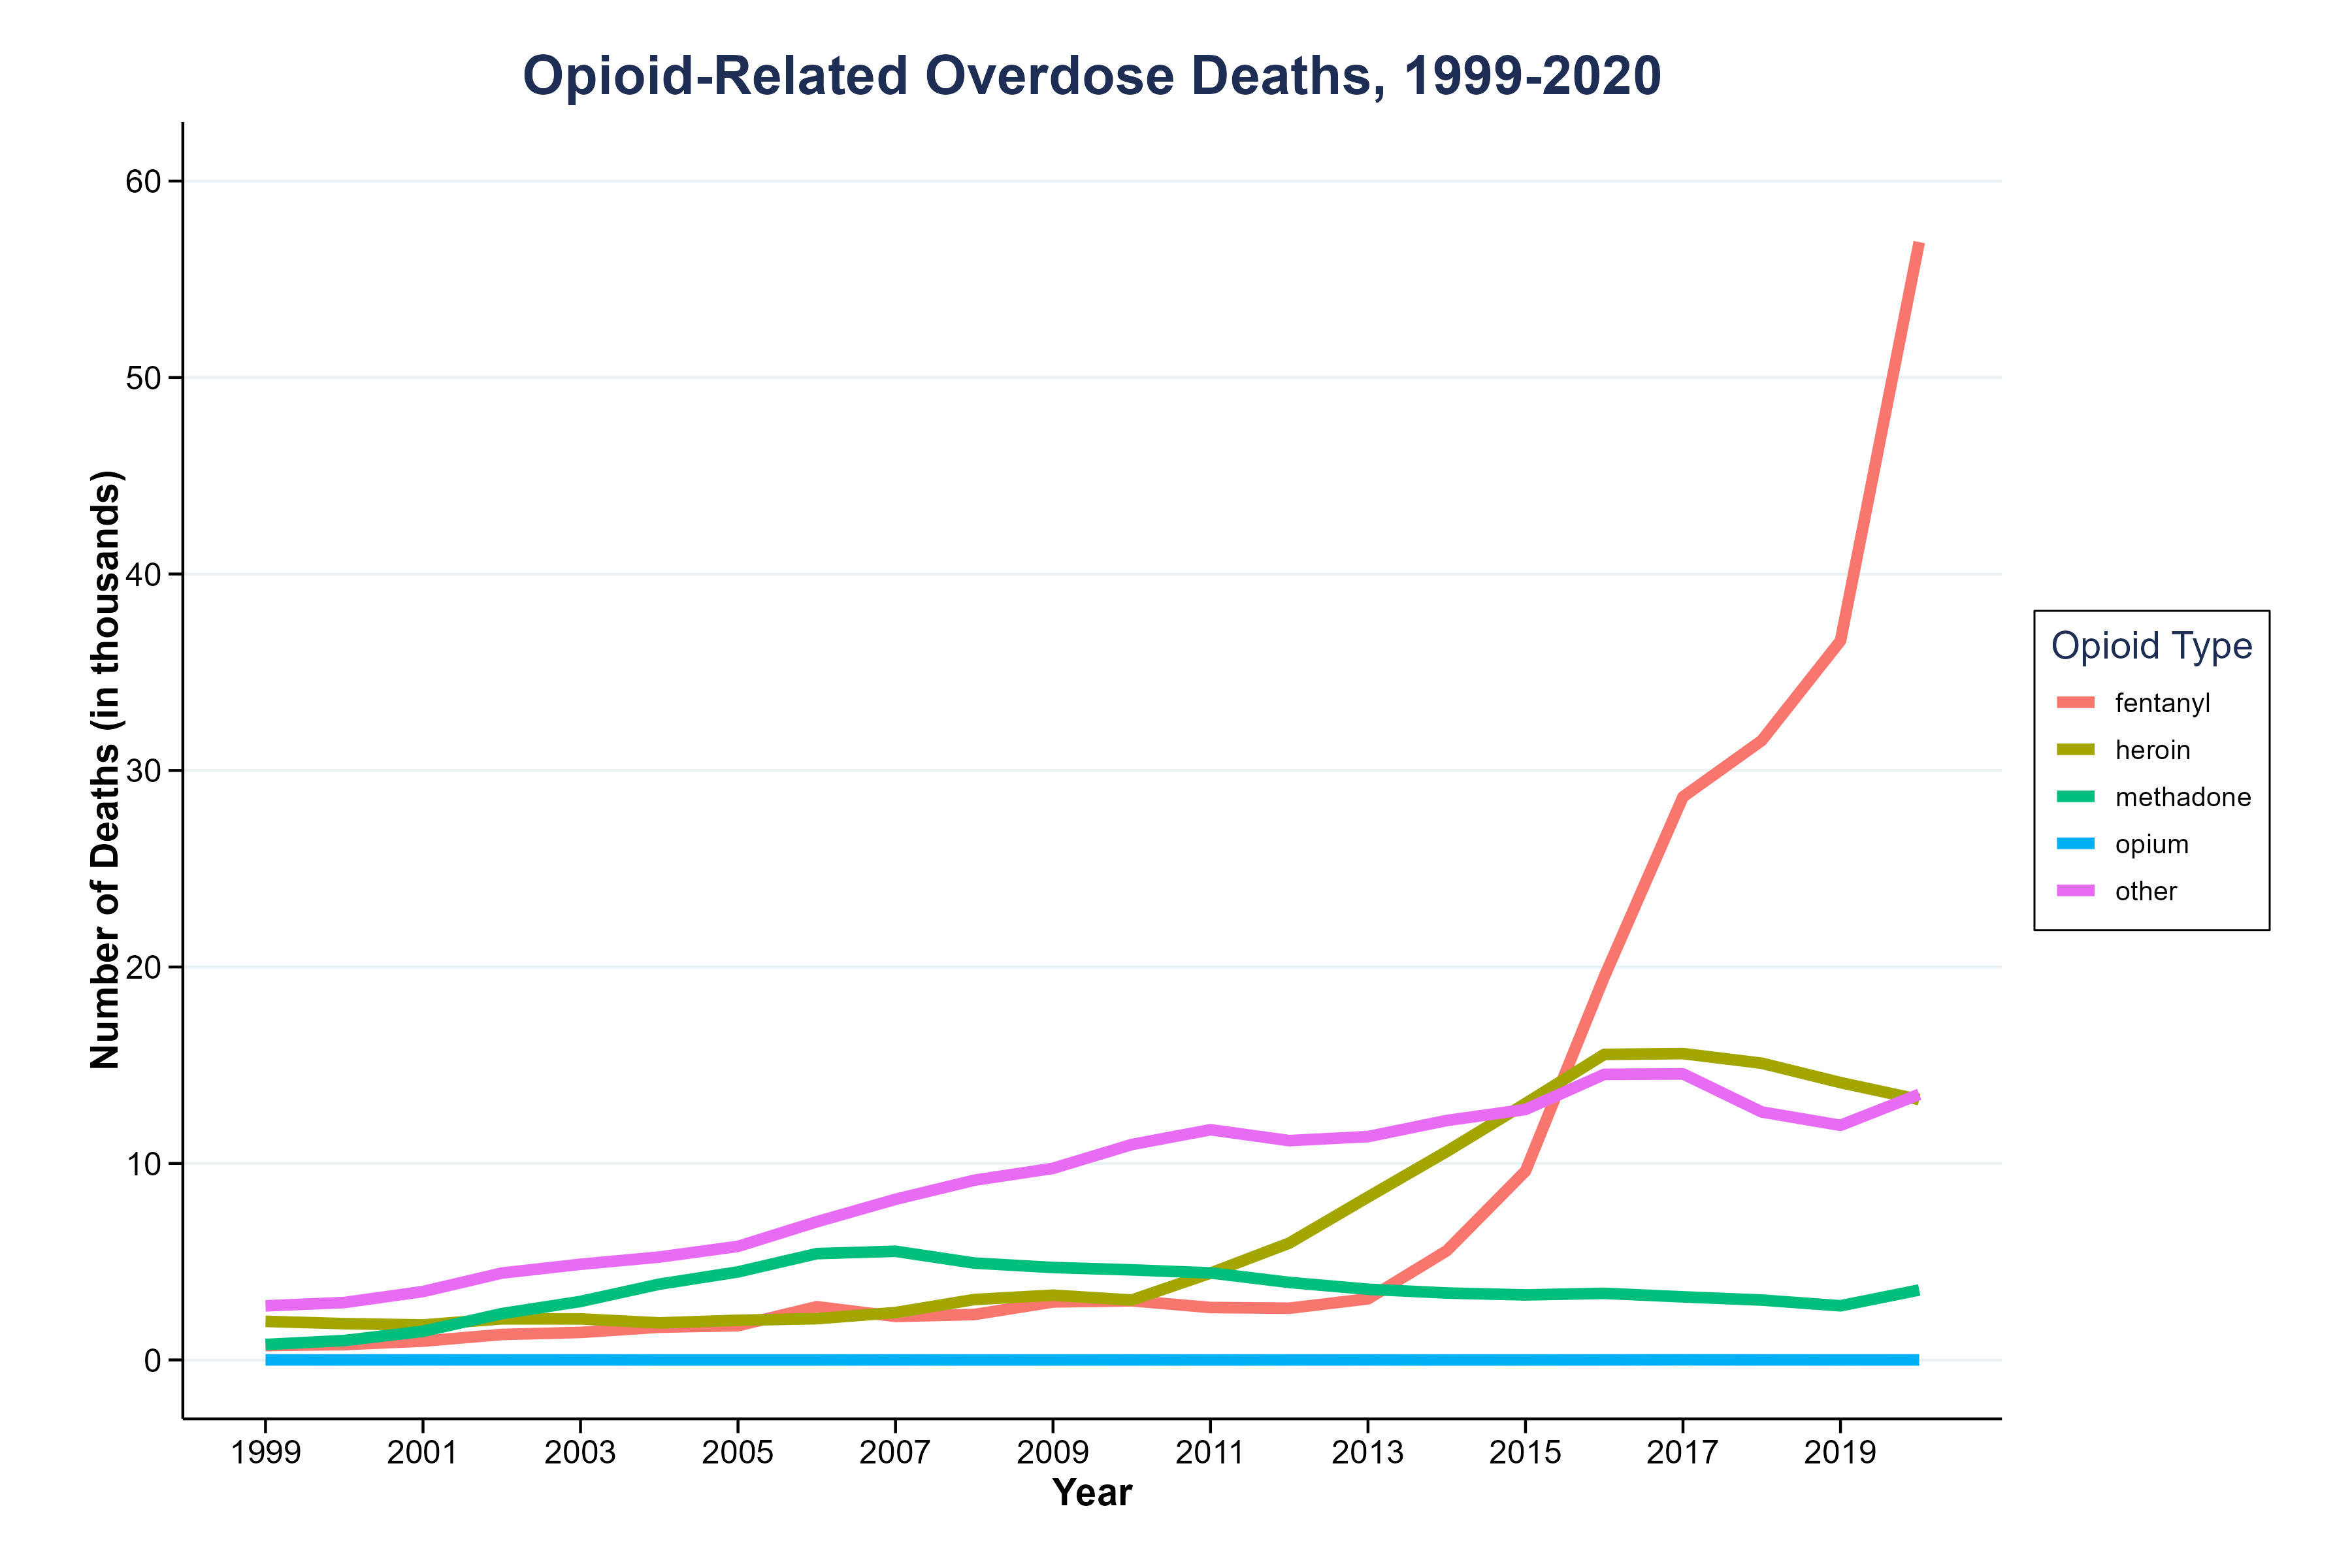
\includegraphics[keepaspectratio]{opioids.png}}

\subsection{Stimulants}\label{stimulants}

\pandocbounded{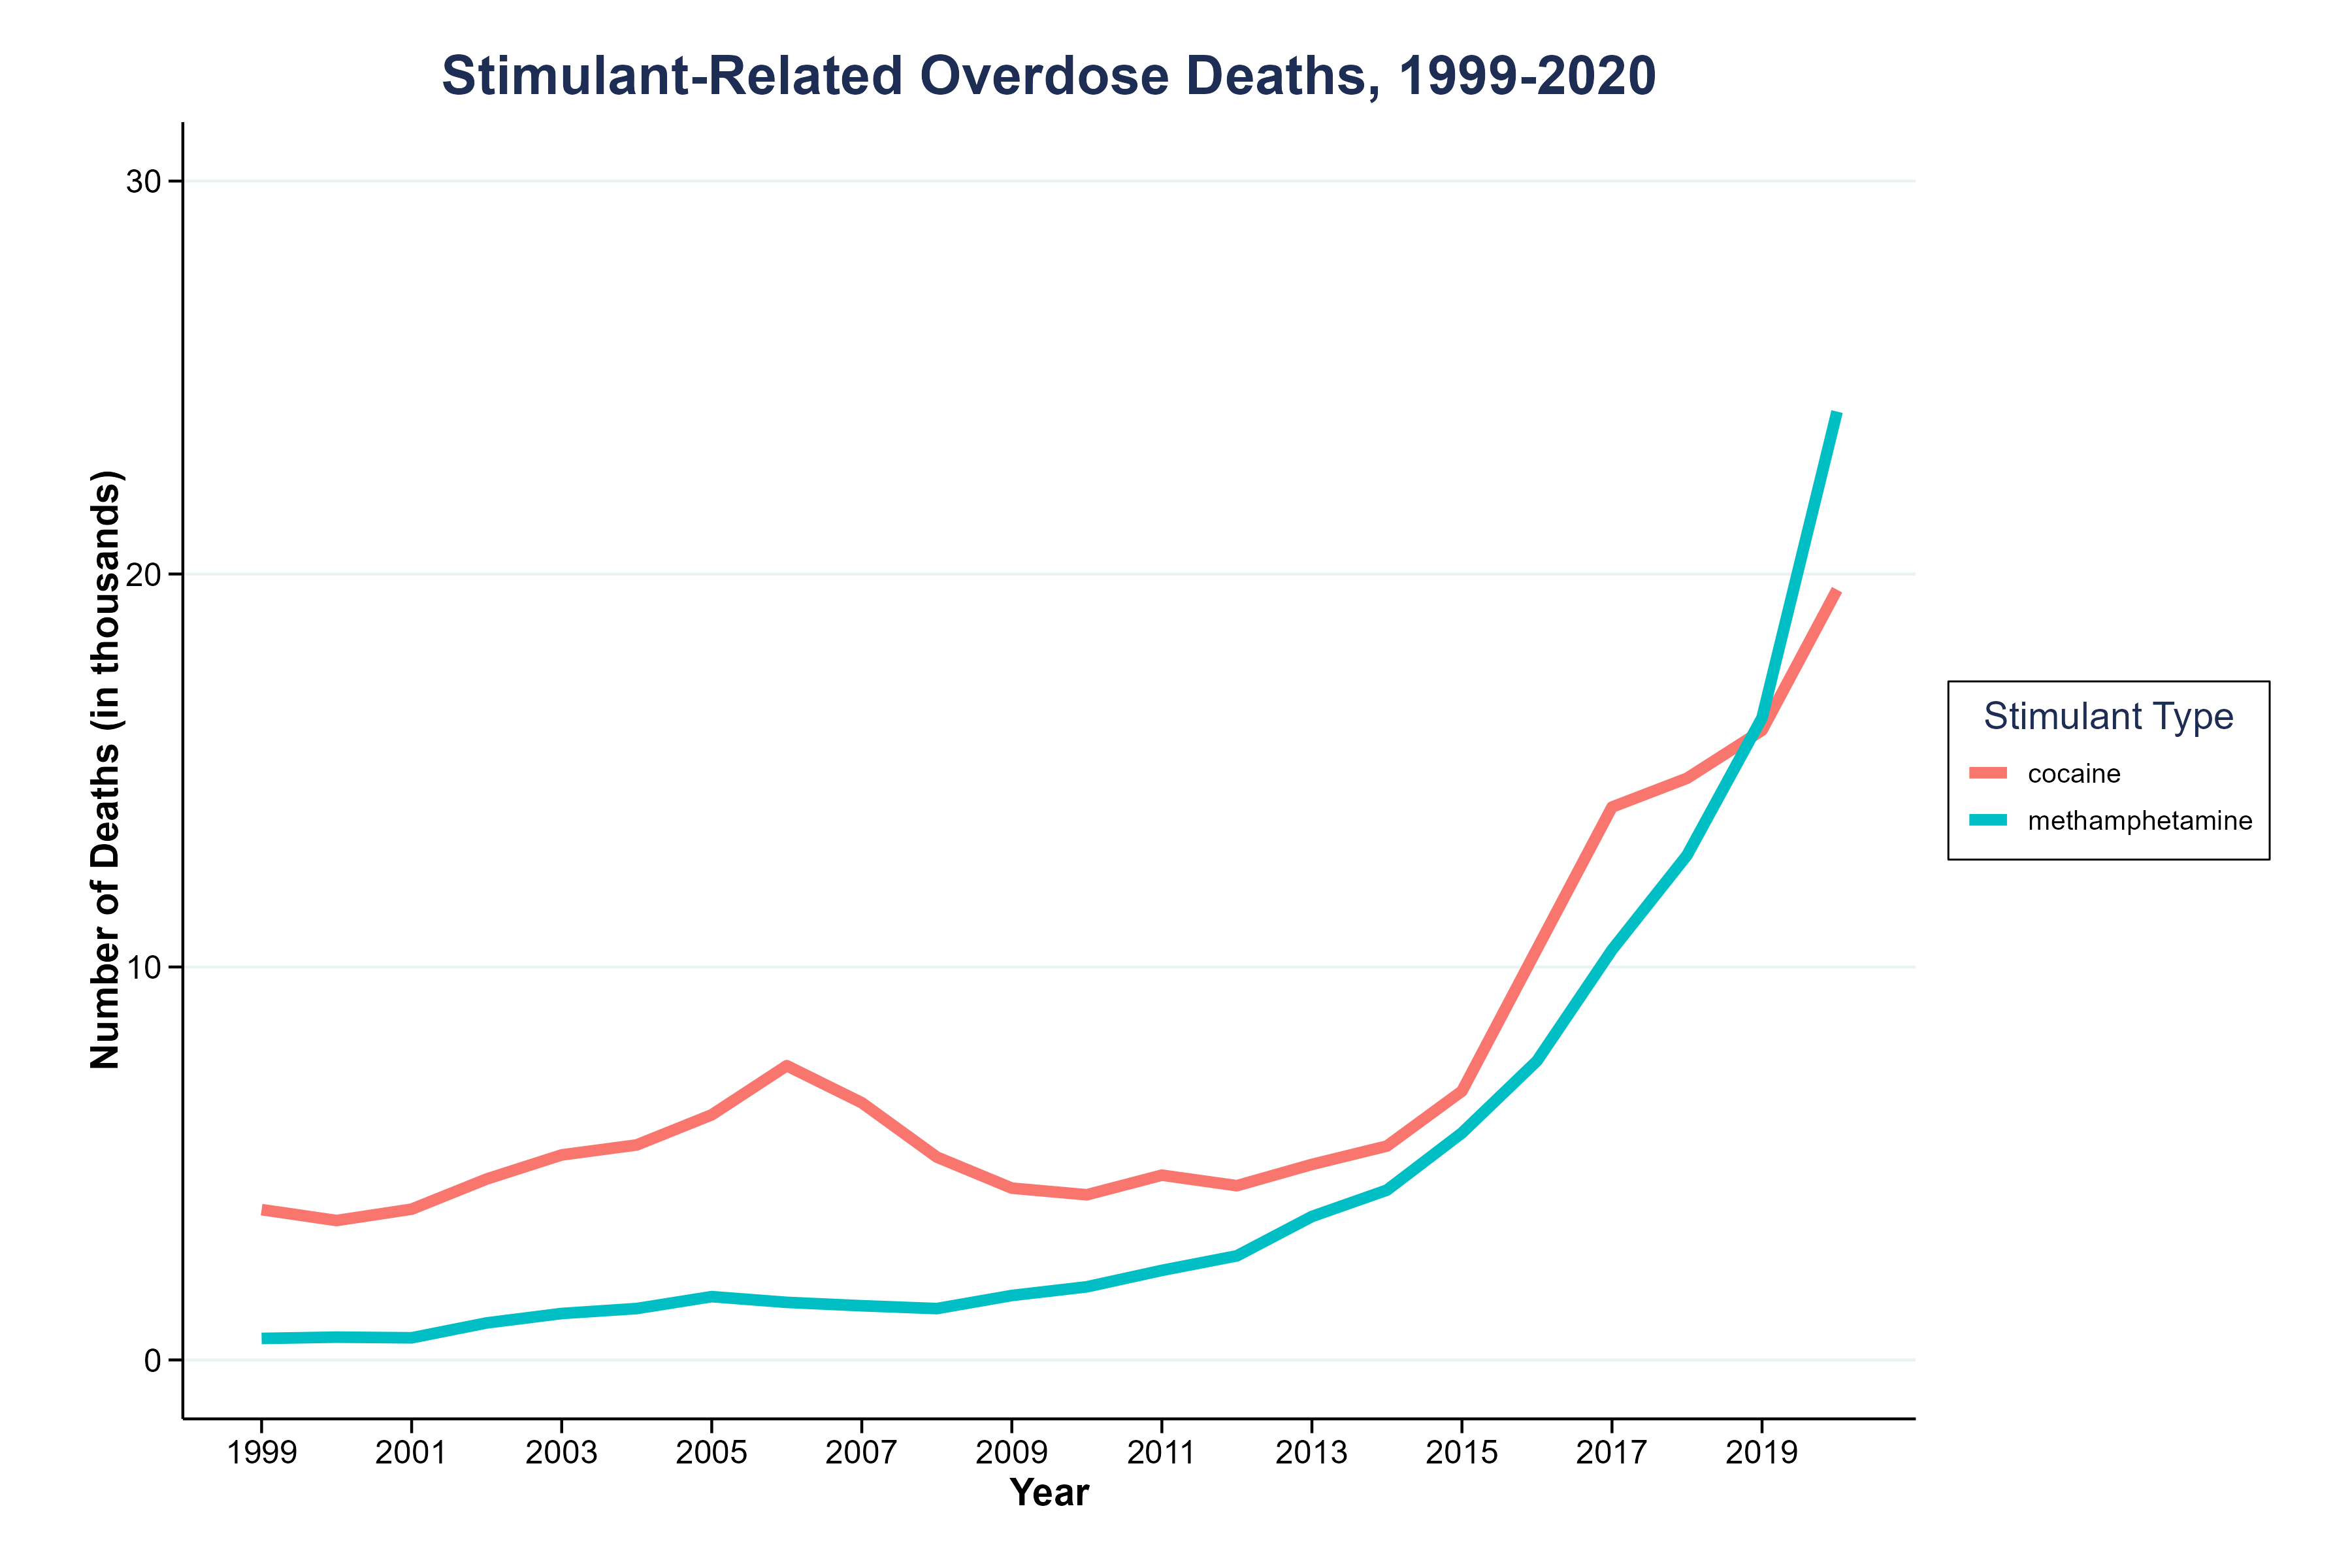
\includegraphics[keepaspectratio]{stimulants.png}}

\subsection{Depressants (non-opioid) /
Sedatives}\label{depressants-non-opioid-sedatives}

\pandocbounded{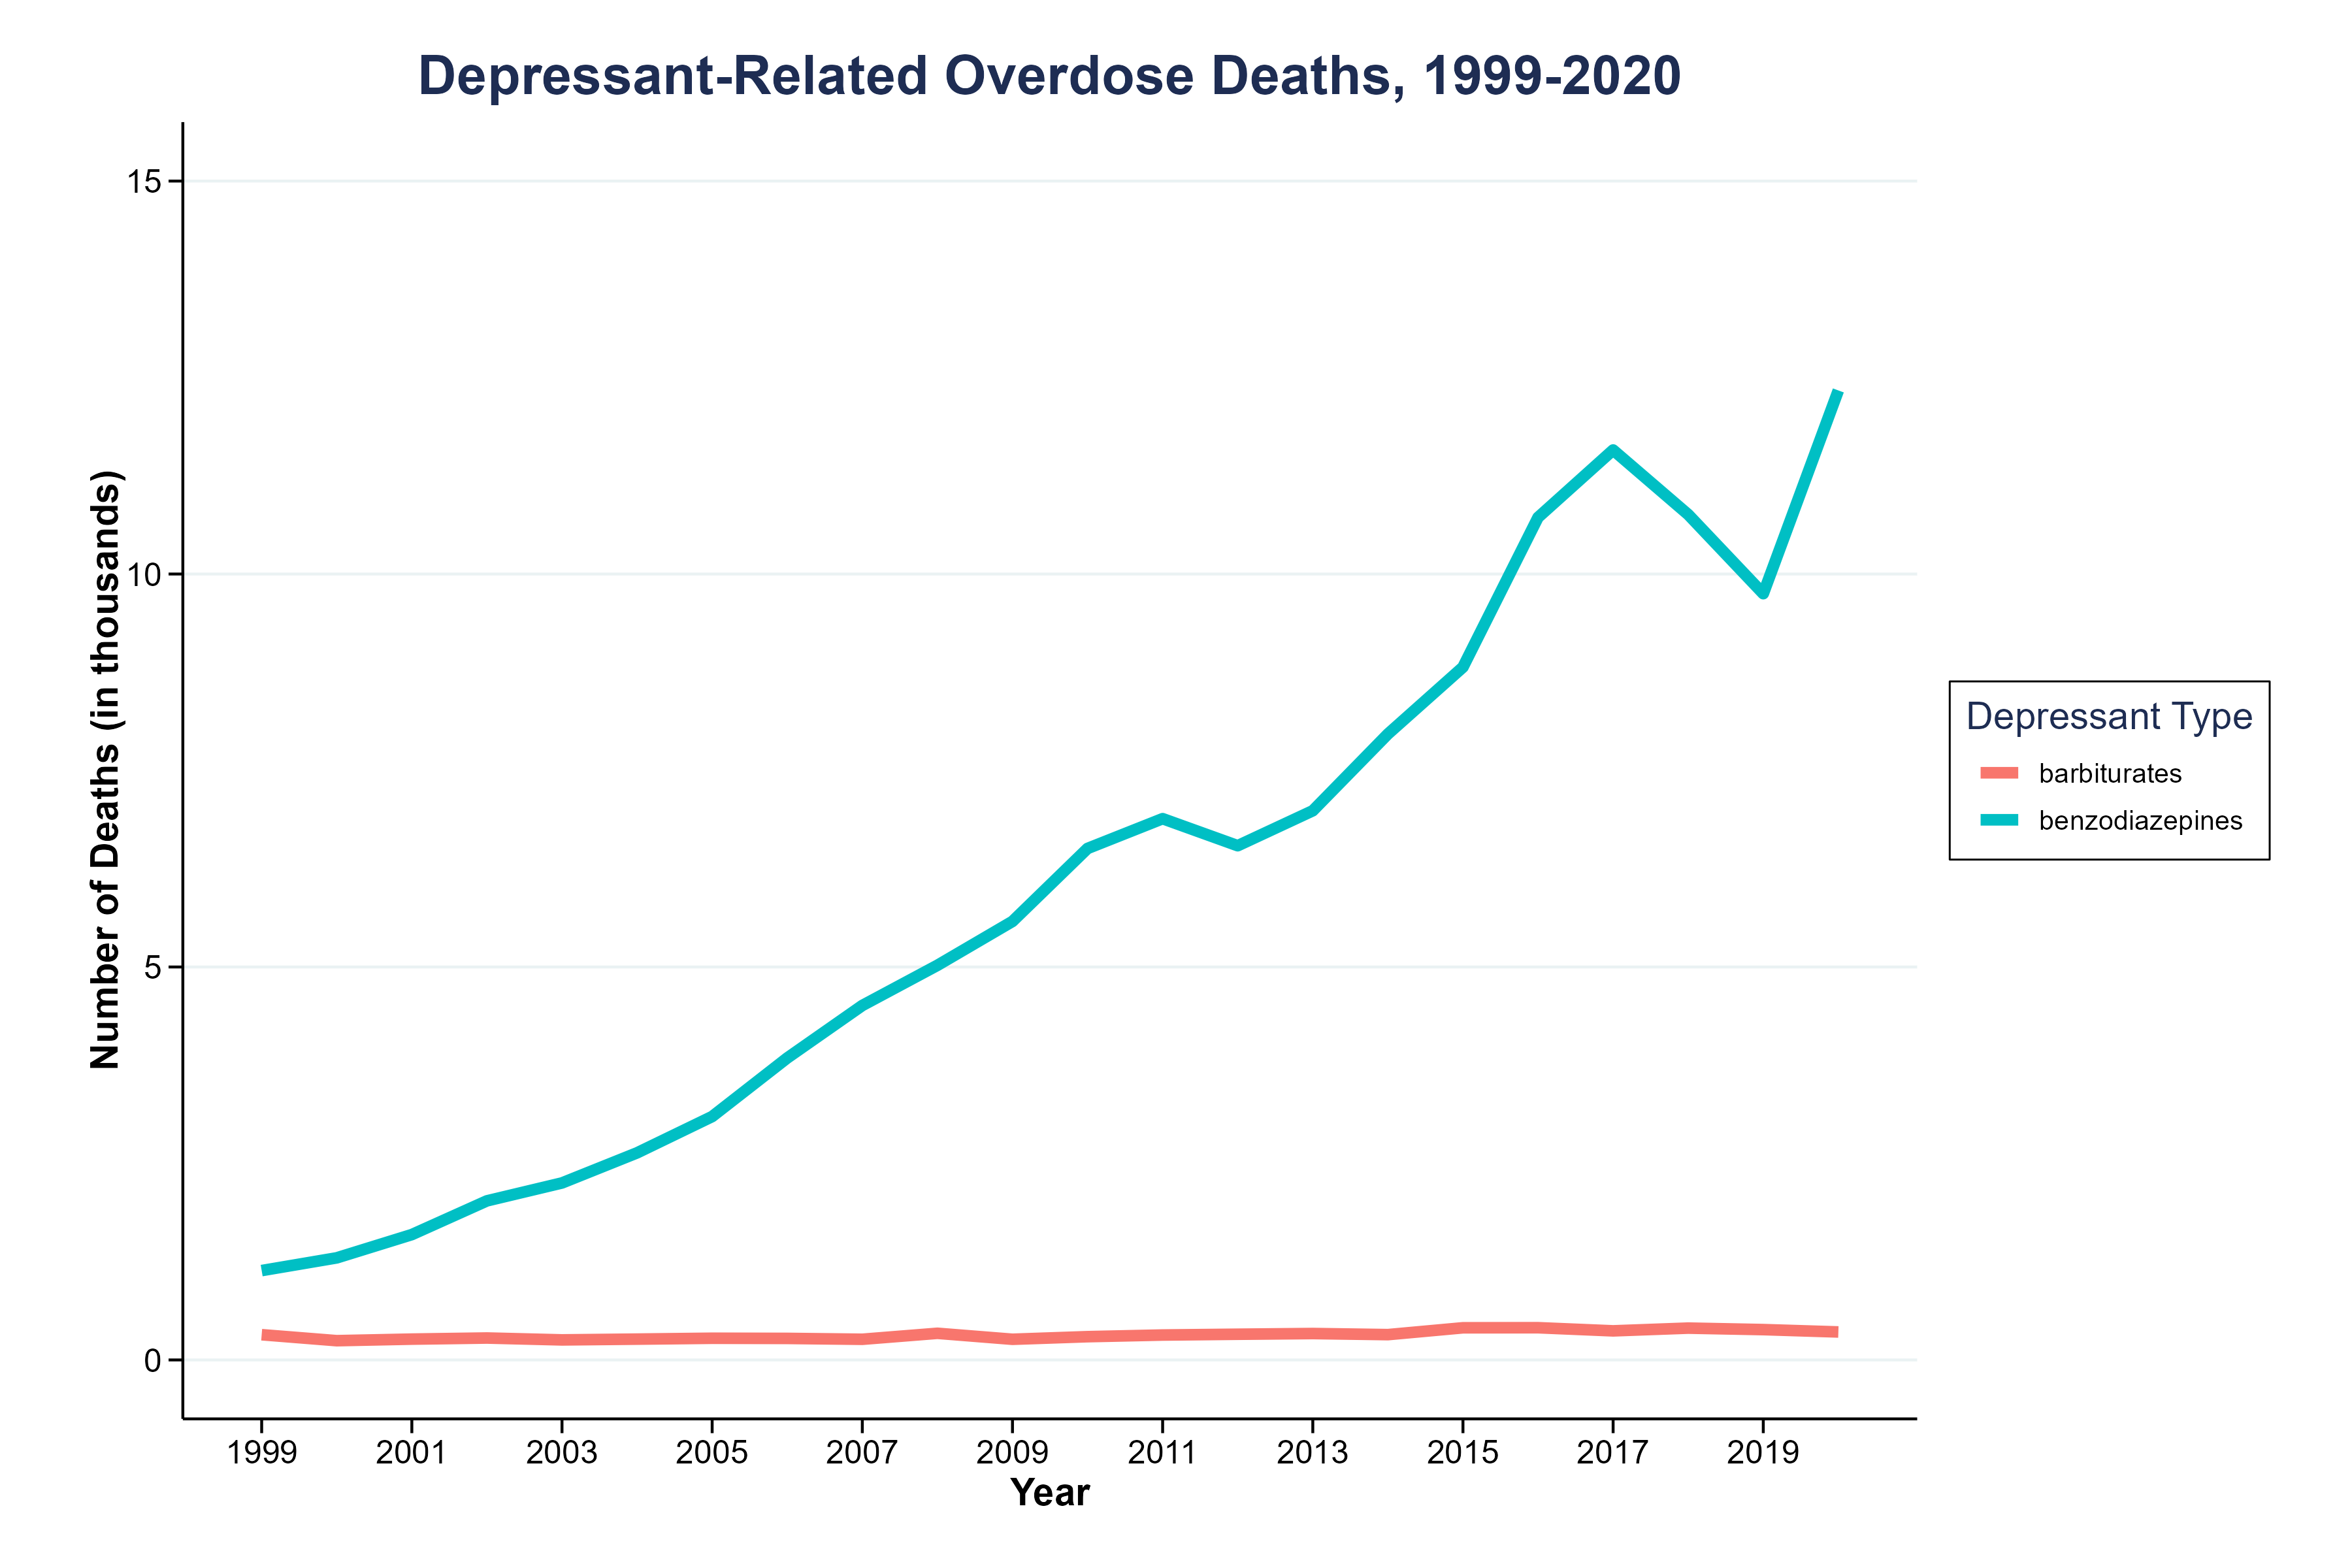
\includegraphics[keepaspectratio]{depressants.png}}

\subsection{Cannabis}\label{cannabis}

\pandocbounded{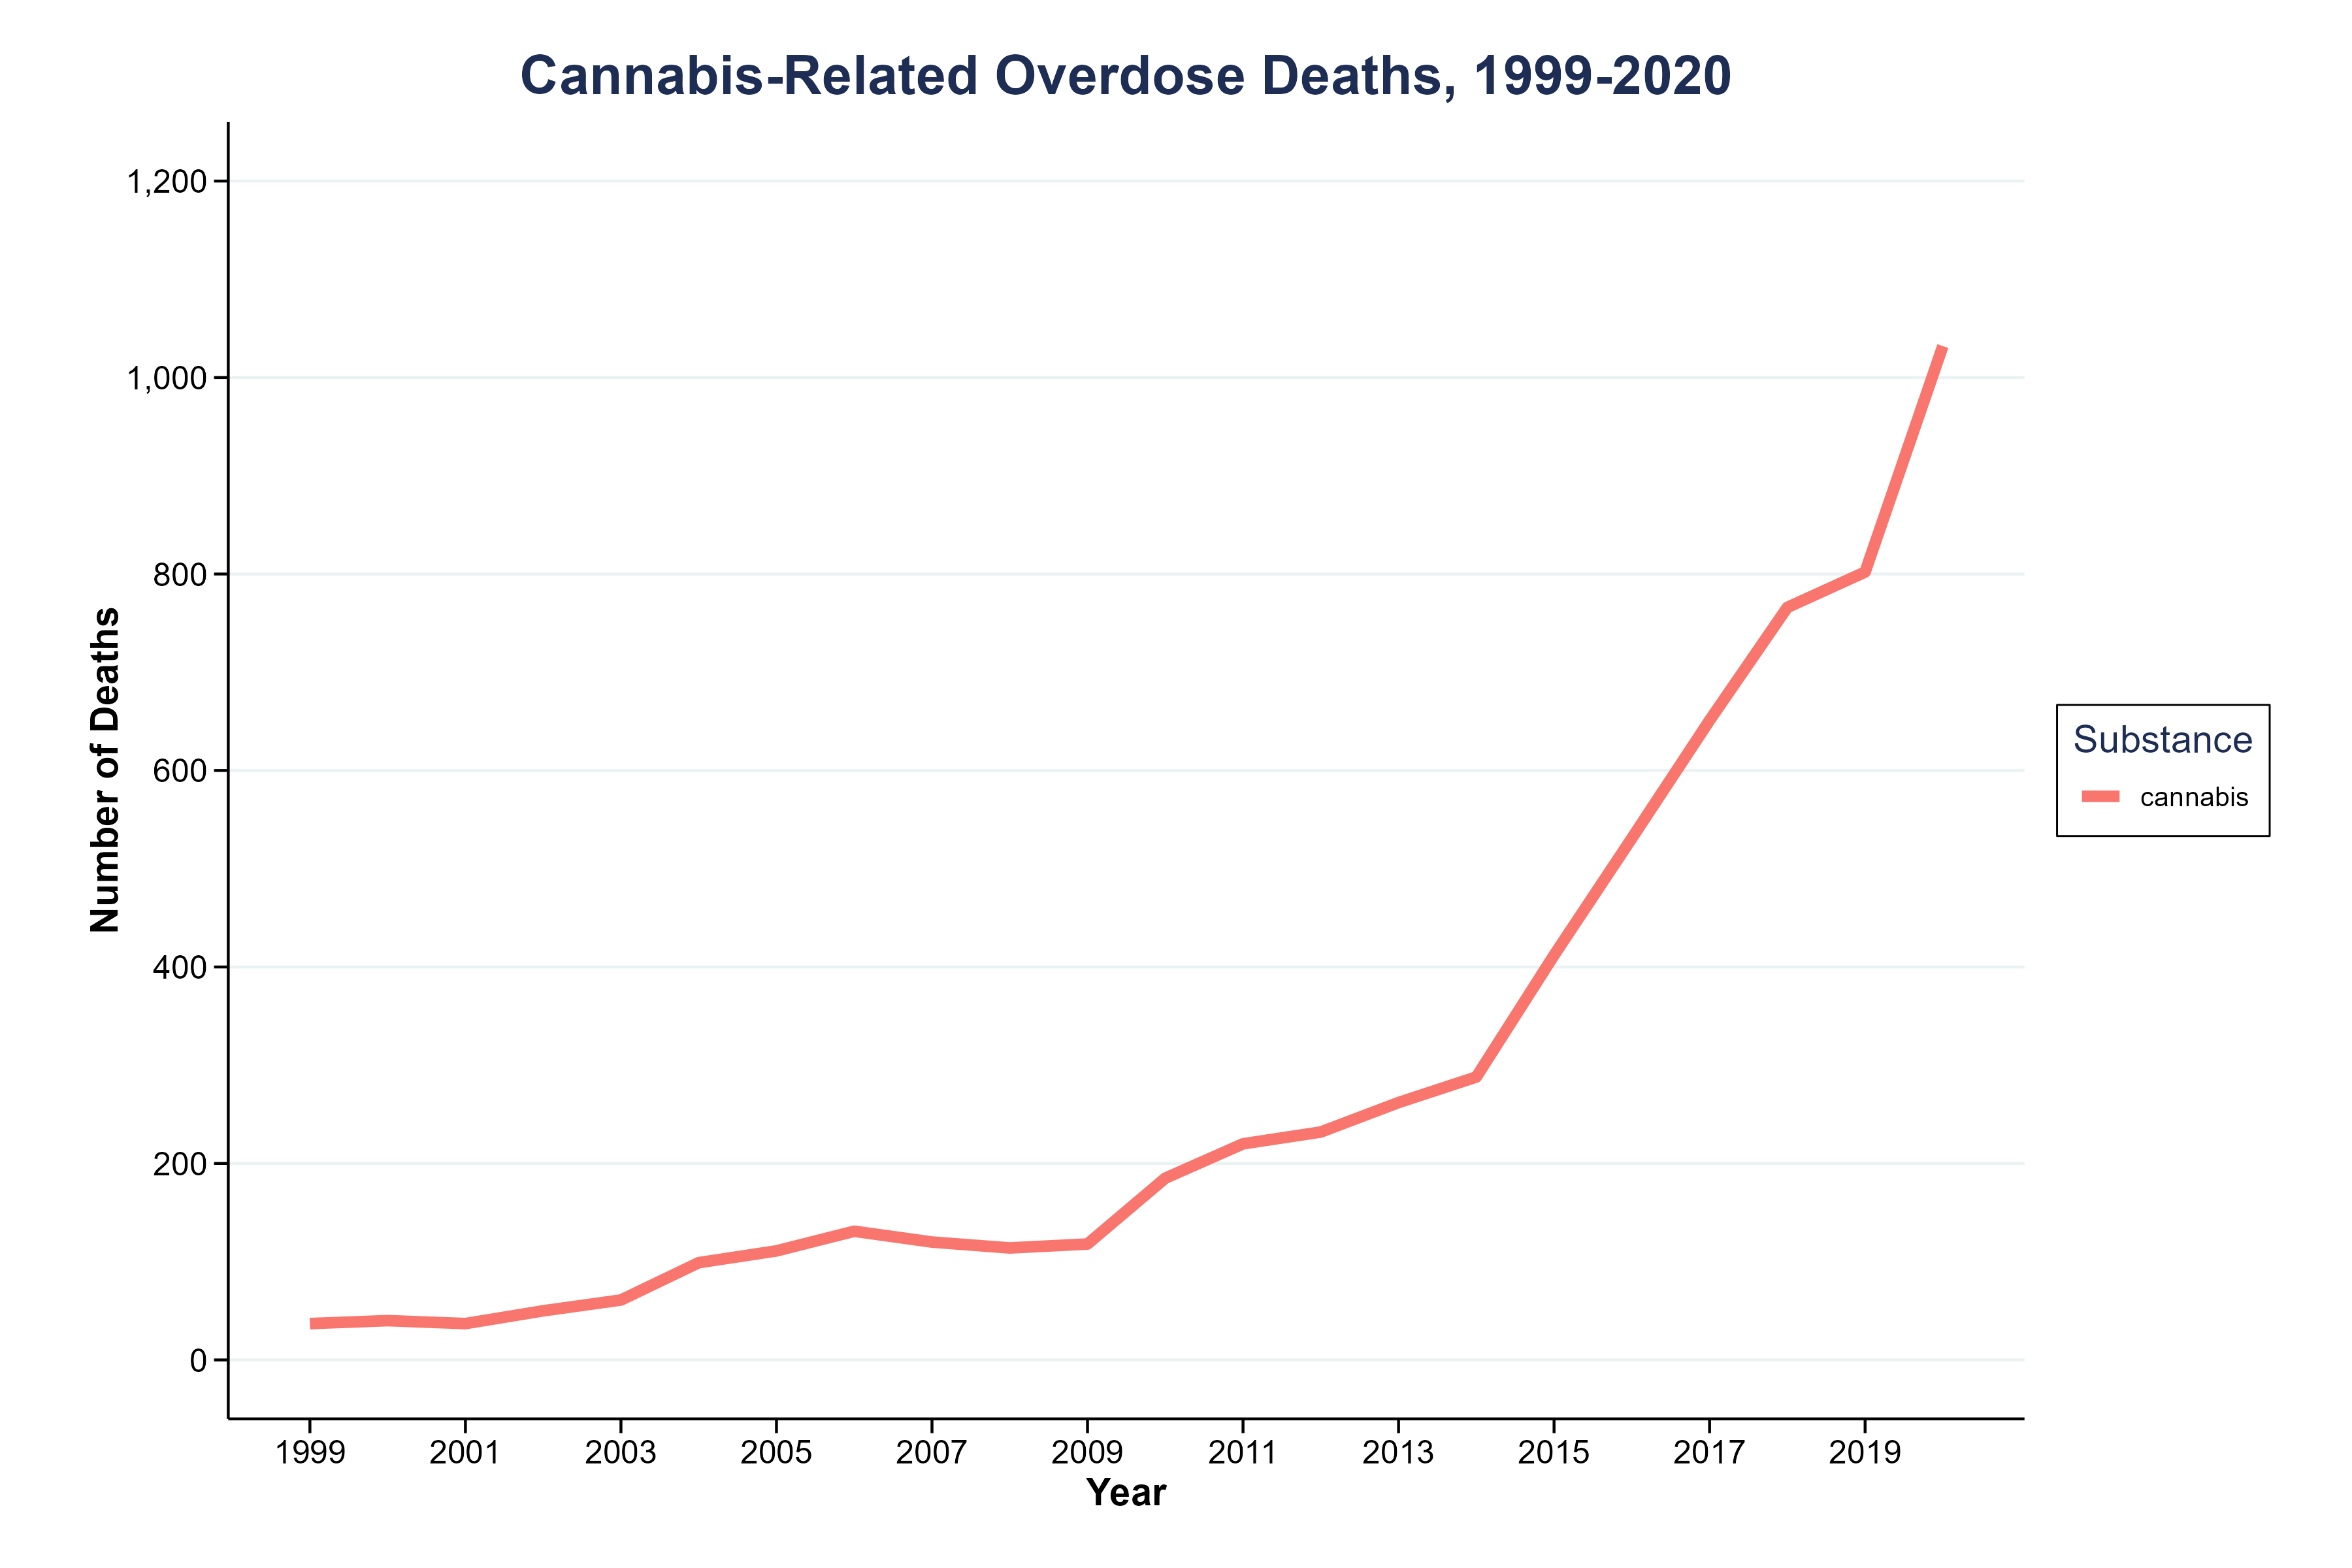
\includegraphics[keepaspectratio]{cannabis.png}}

\subsection{Polysubstance Prevalence}\label{polysubstance-prevalence}

\pandocbounded{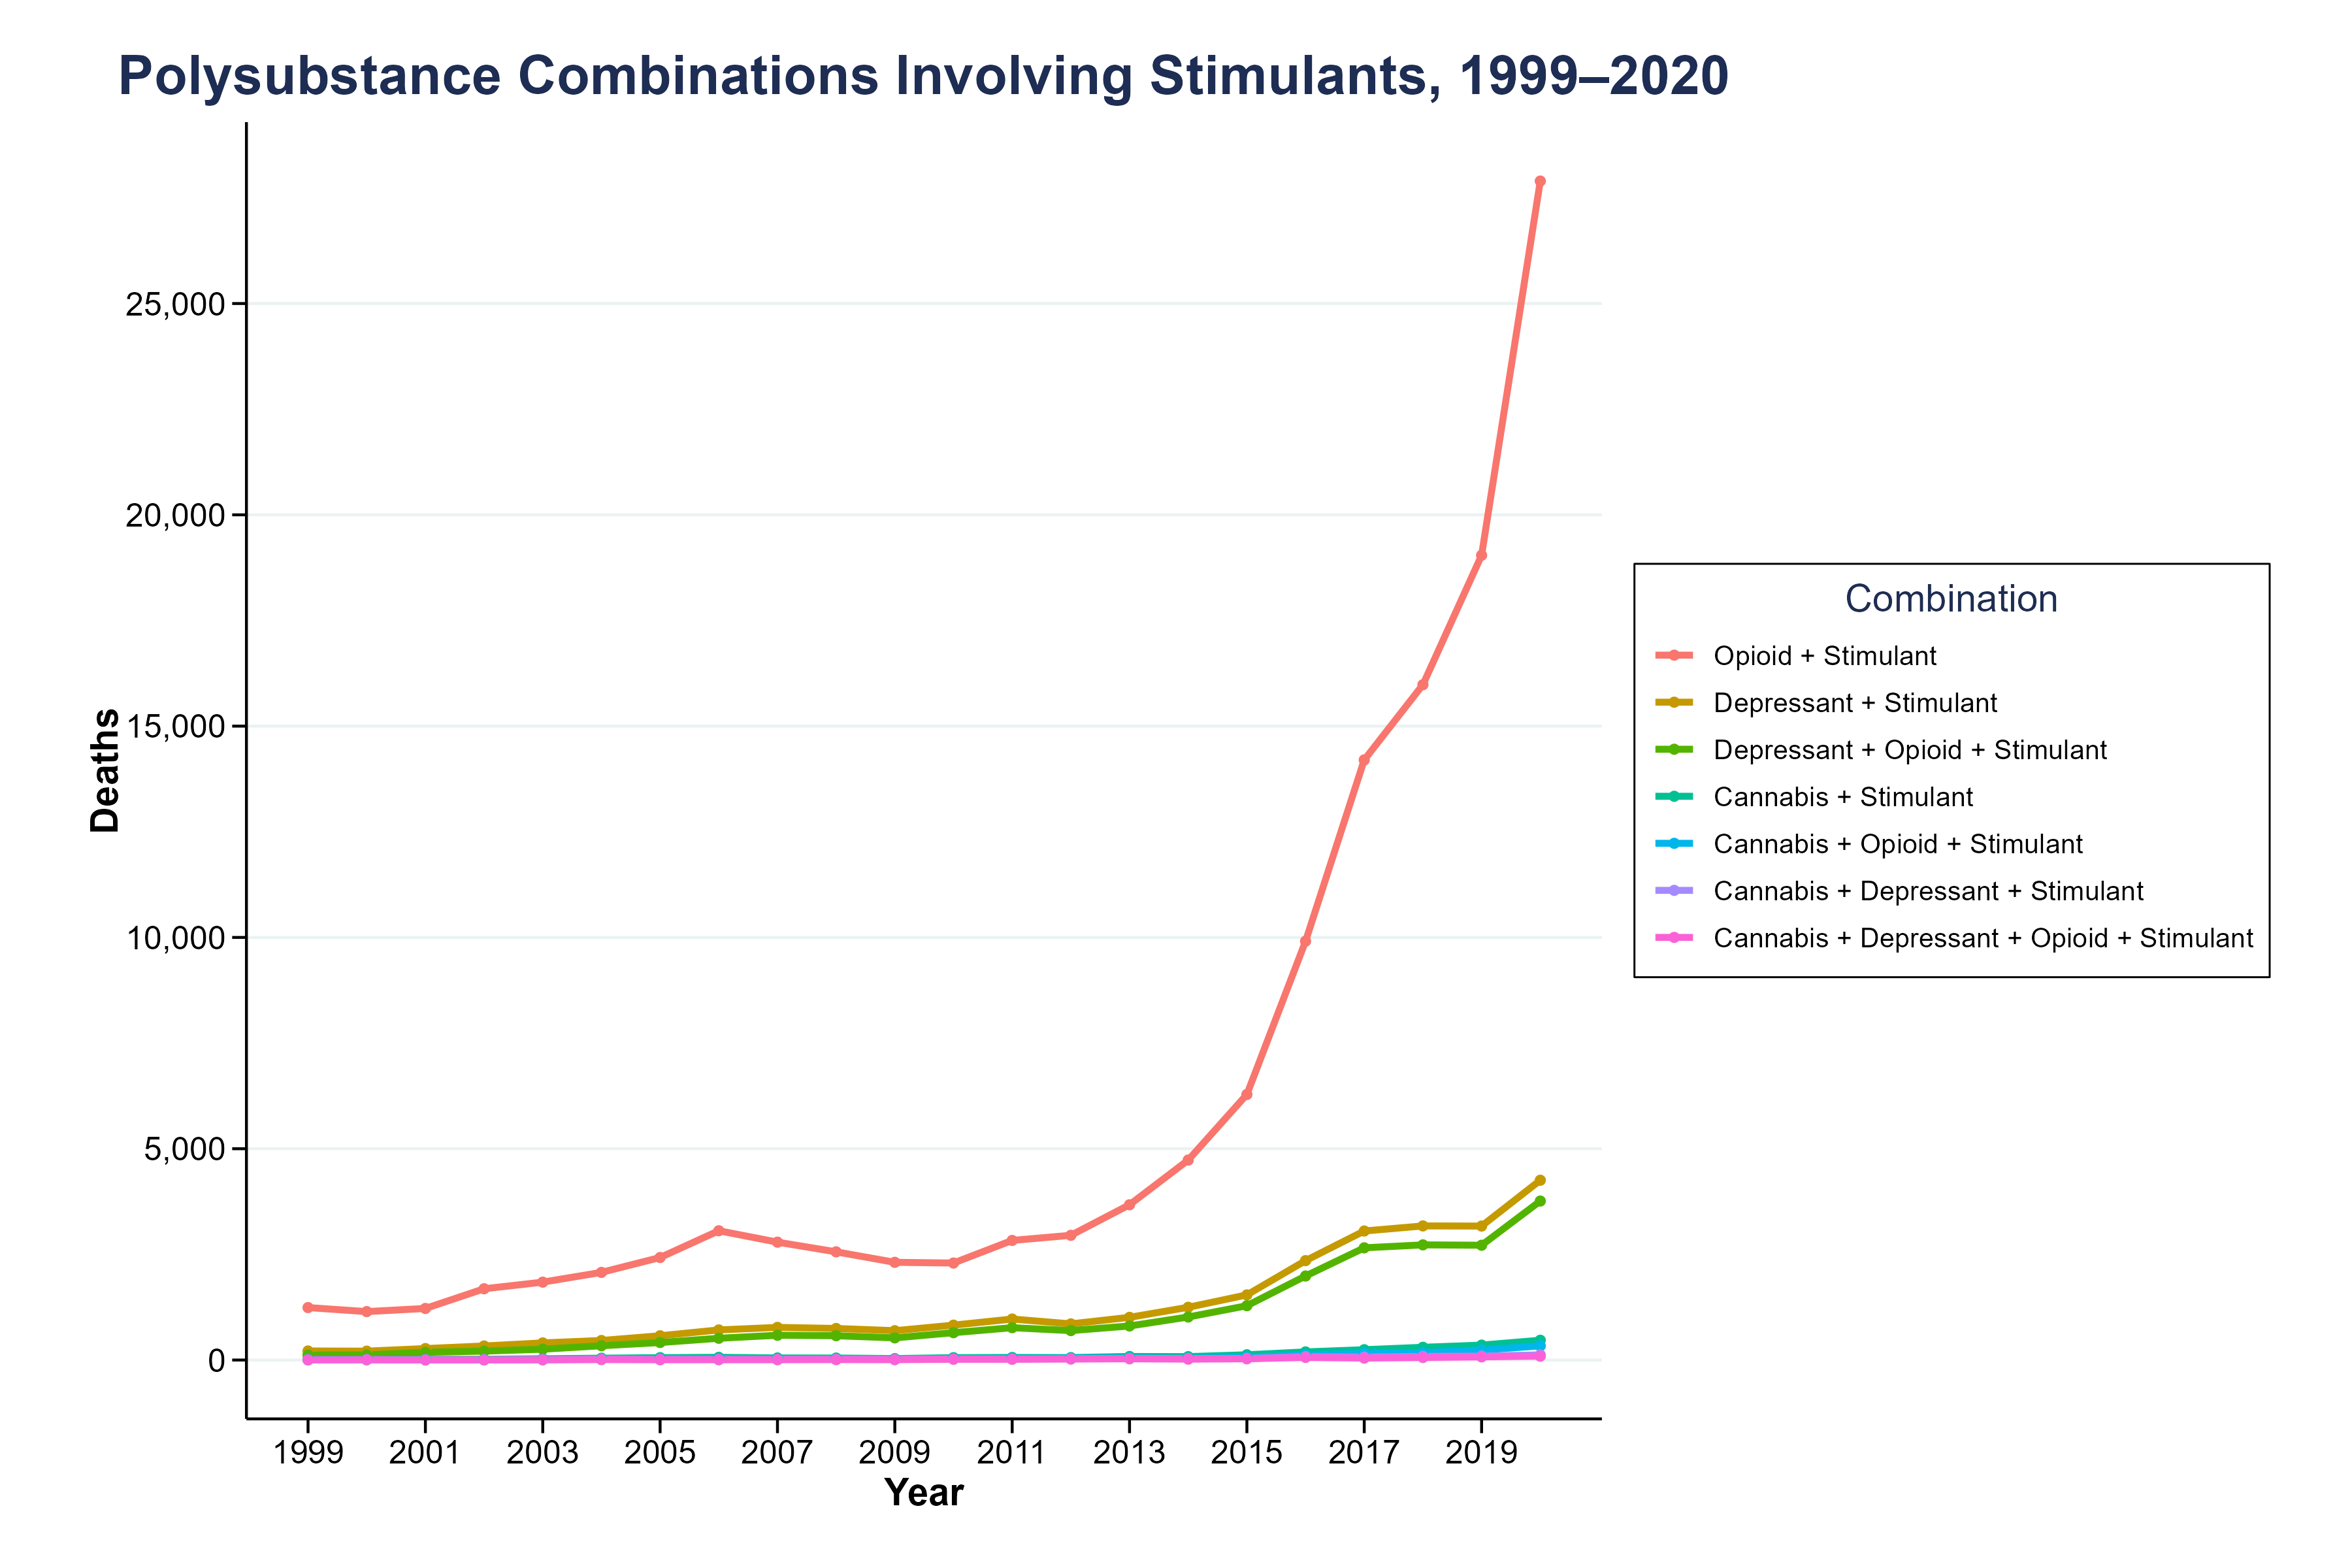
\includegraphics[keepaspectratio]{stimulantcombos.png}}
\pandocbounded{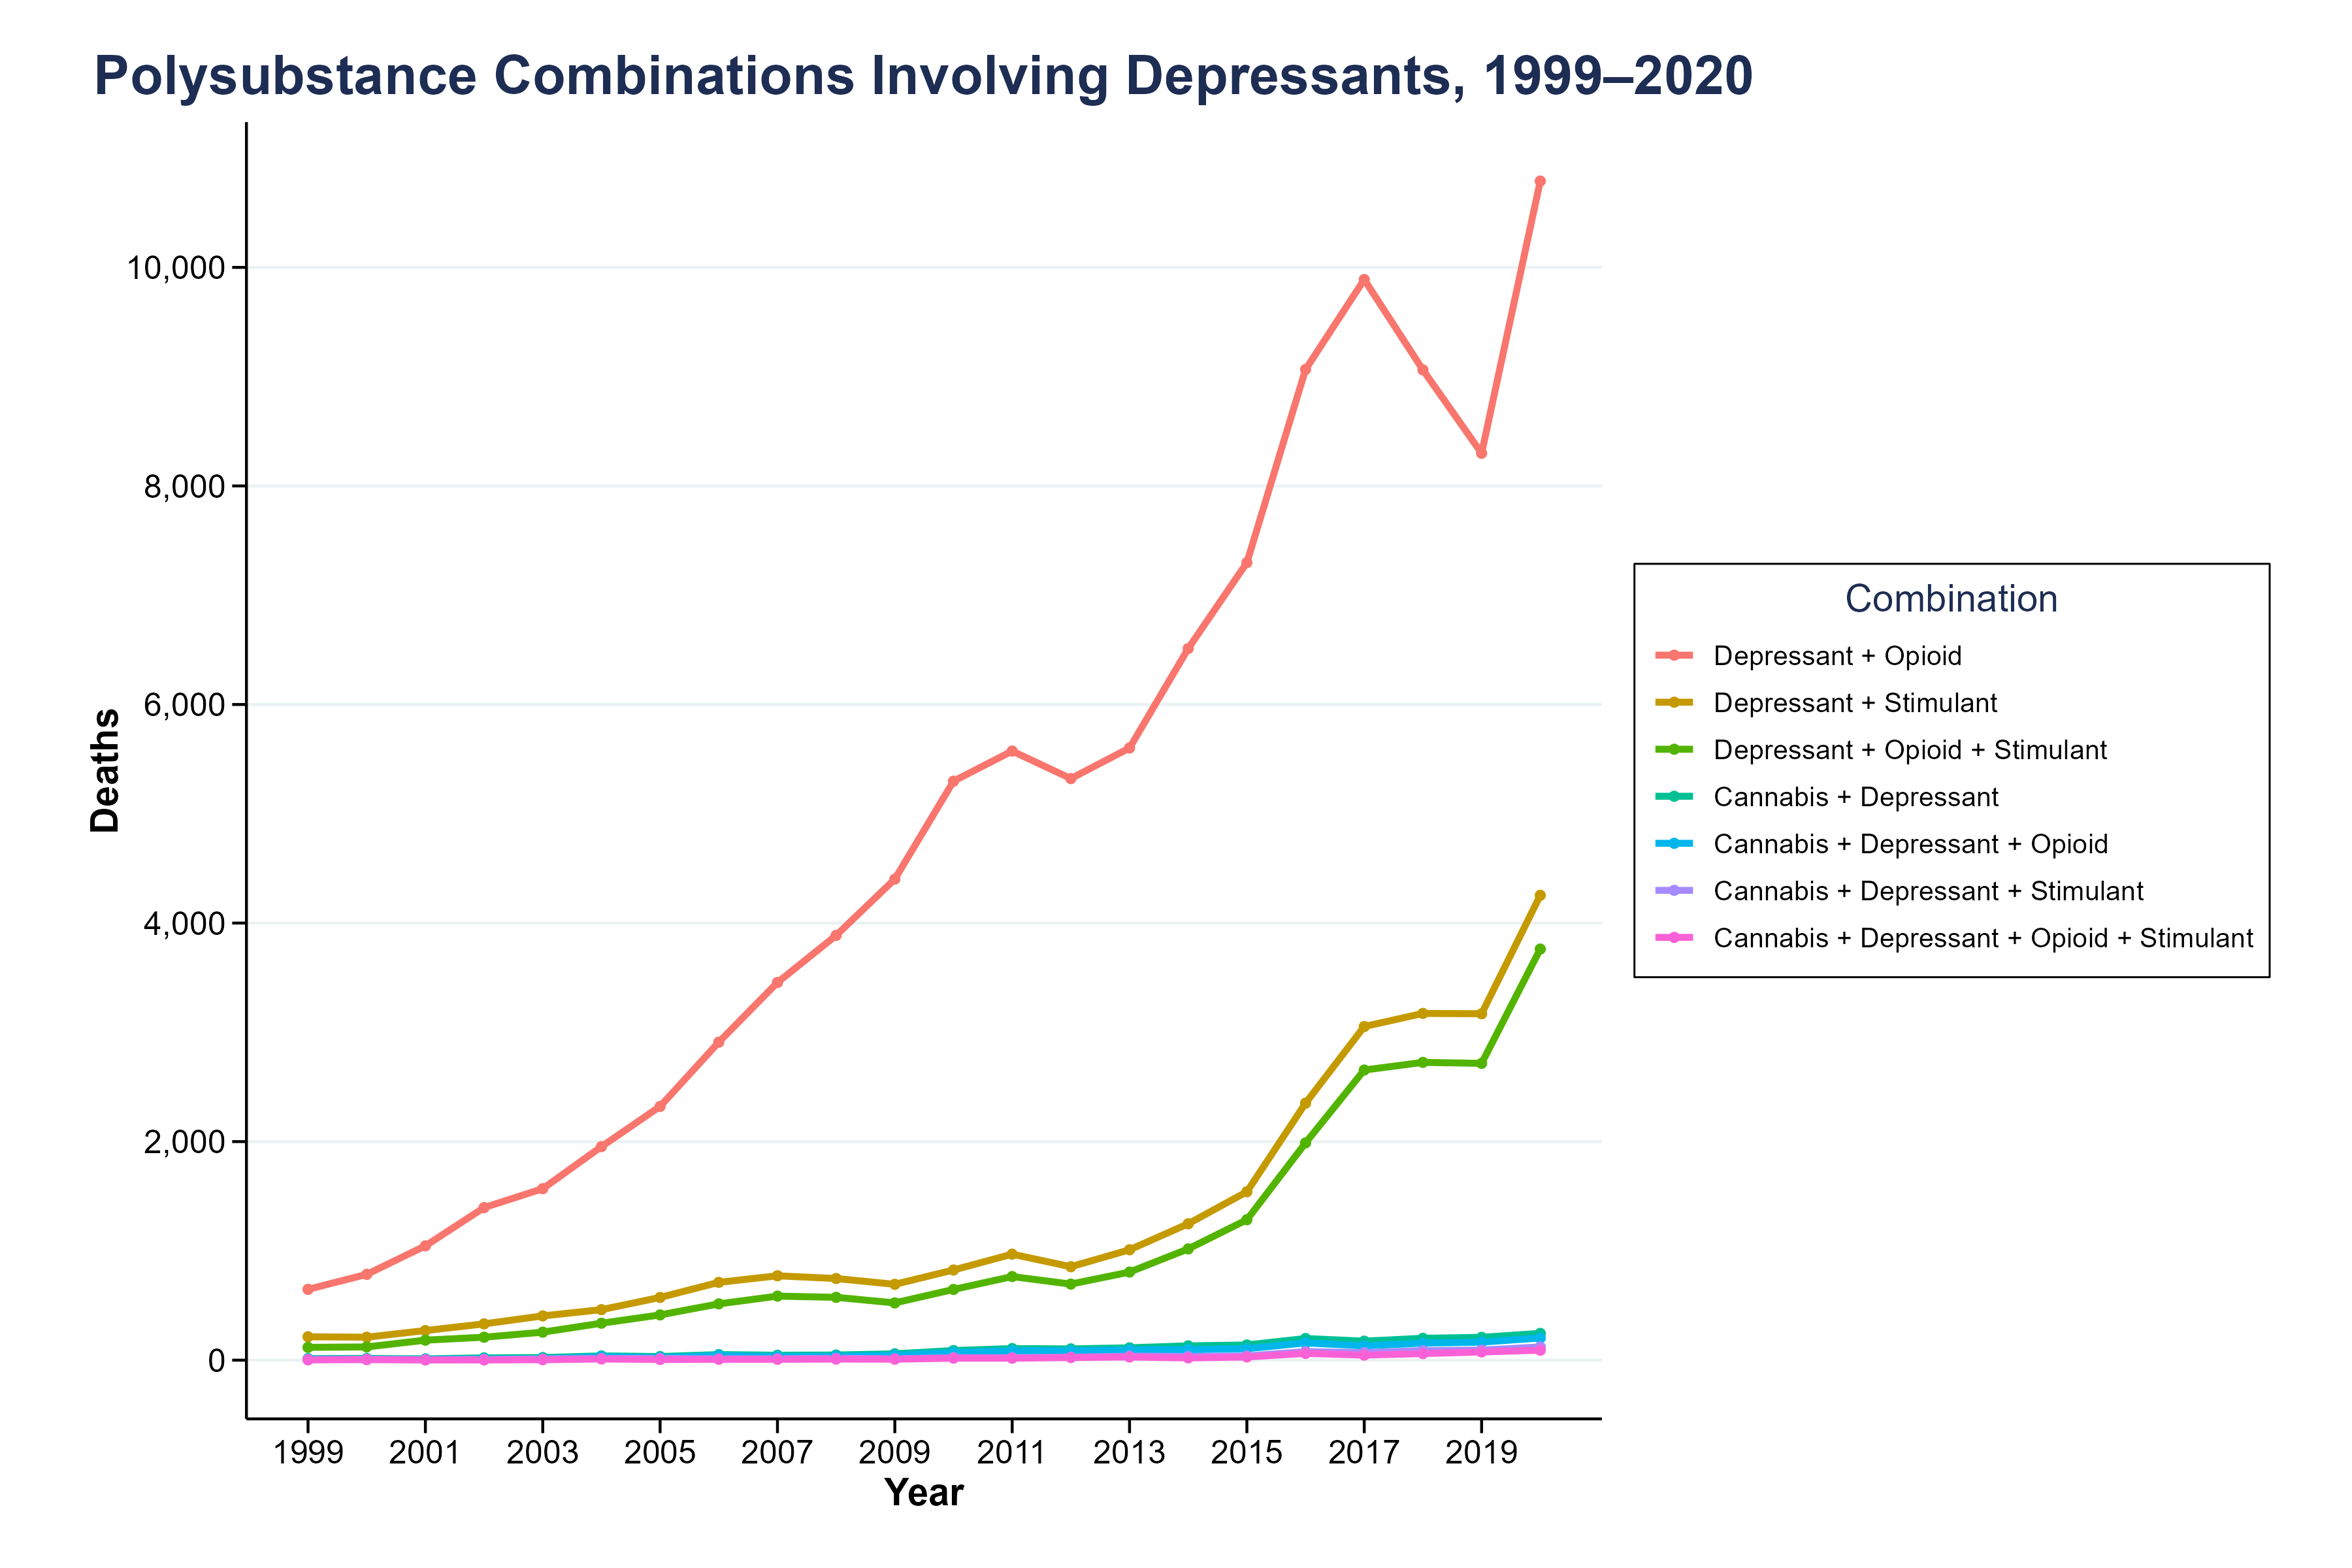
\includegraphics[keepaspectratio]{depressantcombos.png}}
\pandocbounded{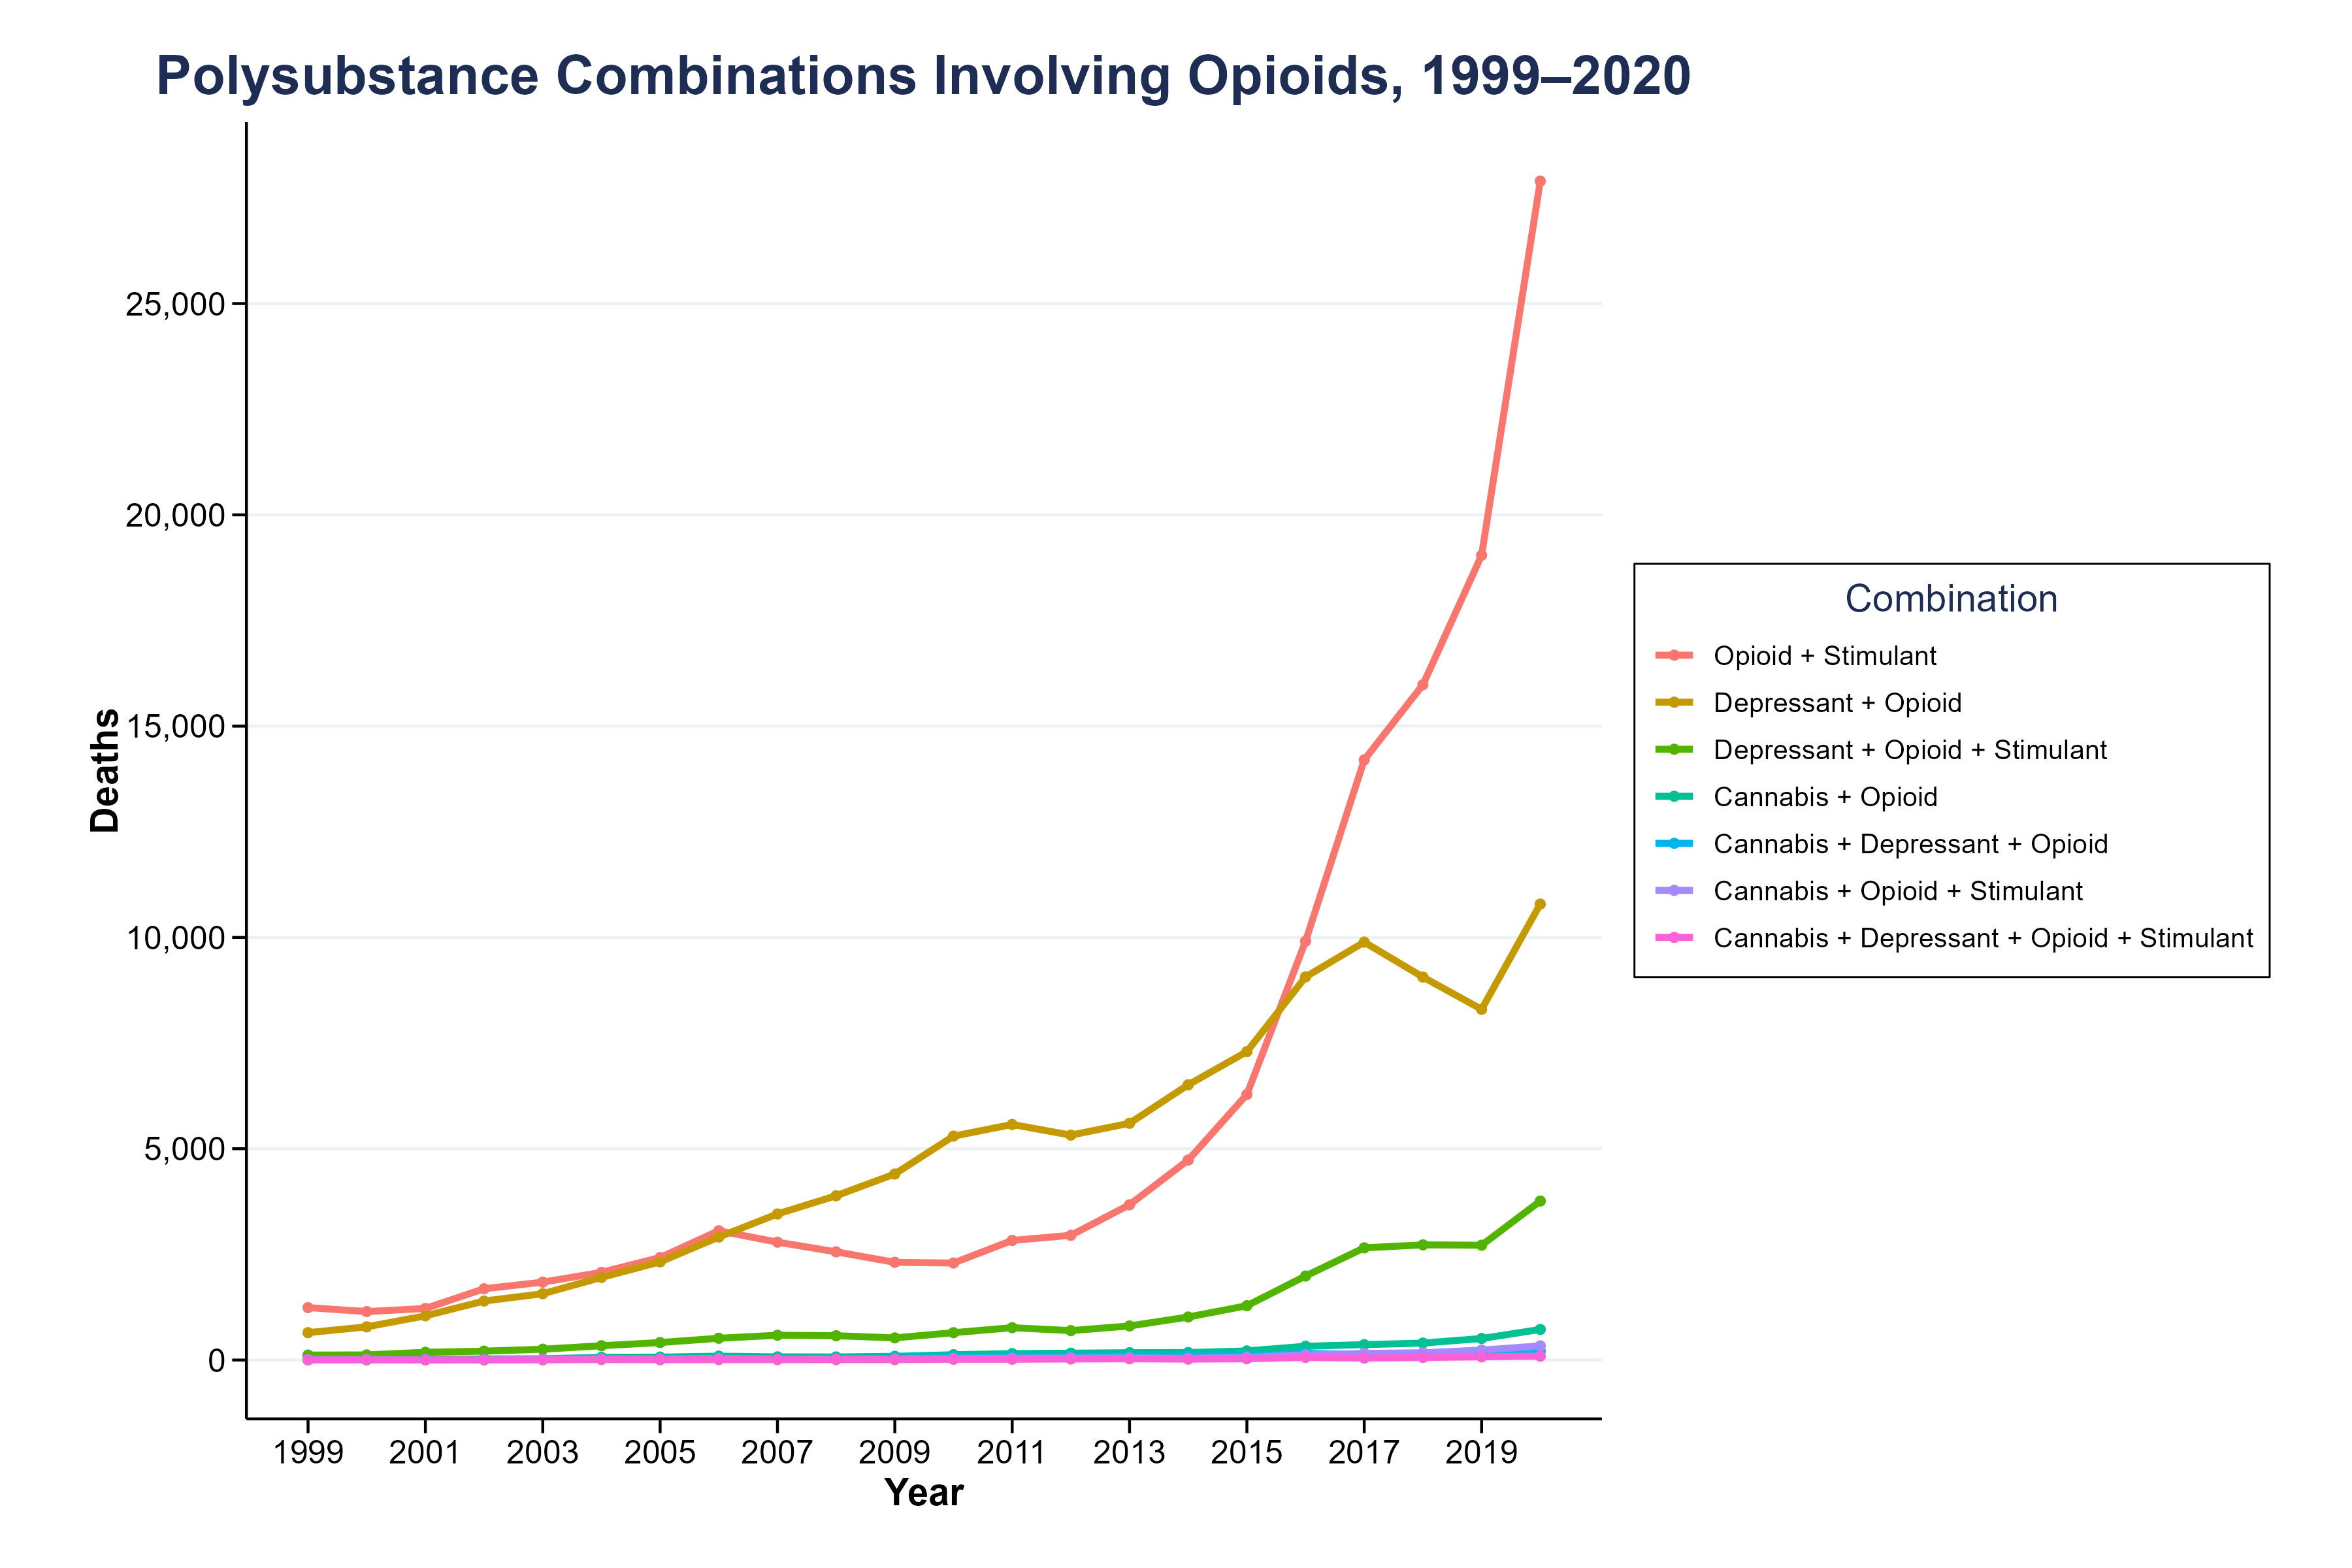
\includegraphics[keepaspectratio]{opioidcombos.png}}

\subsection{Appendix}\label{appendix}

\paragraph{Data Source}\label{data-source}

\href{https://www.nber.org/research/data/mortality-data-vital-statistics-nchs-multiple-cause-death-data}{NBER/NVSS
Multiple Cause-of-Death Data}

\begin{itemize}
\tightlist
\item
  Multiple Cause-of-death Mortality Data from the National Vital
  Statistics System (NVSS) of the National Center for Health Statistics
  (NCHS)
\item
  National Bureau of Economic Research Public Use Data Archive
\item
  Downloaded on 4 September 2025
\end{itemize}

\paragraph{International Statistical Classification of Diseases and
Related Health Problems 10th Revision
(ICD-10)}\label{international-statistical-classification-of-diseases-and-related-health-problems-10th-revision-icd-10}

\href{https://icd.who.int/browse10/2019/en}{ICD-10 Classification
(2019)}




\end{document}
